% LaTeX file for Chapter 03


\chapter{Results}

\section{Exploratory Data Analysis}

\subsection{Mouse kidney cells} \label{mouse_dataset}
The first data set stems from a paper that investigates potential cellular targets of kidney disease in mice \citep{mouse_cells}. The authors isolated and sequenced a total of 57'979 cells from whole kidney cell suspensions (one kidney per mouse) derived from seven healthy male mice using droplet-based single-cell RNA sequencing. The samples were labelled as: normal1, normal2, normal3, normal4, Ksp-cre-GFP, Scl-cre-GFP and Pod-cre-GFP. For our work, we decided to use the raw data from the four samples that were labelled as normal to ensure the biological reproducibility between the samples.

We used the \emph{alevin-fry} pipeline to quantify the raw single-cell RNA sequencing data for further use in the R programming environment. Quality control is a crucial stage in data pre-processing as low-quality libraries can contribute to misleading results in downstream analyses \citep{OSCA}. Therefore, we filtered lowly abundant genes and low-quality cells to mitigate said problems to improve interpretability of the results. 

To identify low-quality cells, cell-specific QC metrics were calculated with the \emph{perCellQCMetrics} function from the \emph{scater} R package \citep{scater}. These metrics include the total number of expressed genes, the overall count across all genes, and the fraction of counts assigned to control genes such as mitochondrial genes. By setting a specific threshold on per-cell QC metrics, high-quality cells can be retained. In our setting, outliers are defined as cells with library sizes more than two median absolute deviations away from the median library size. Figure \ref{fig:QC} summarizes the process from unprocessed to processed single-cell experiment. 

\begin{figure}[!htb]
\begin{center}
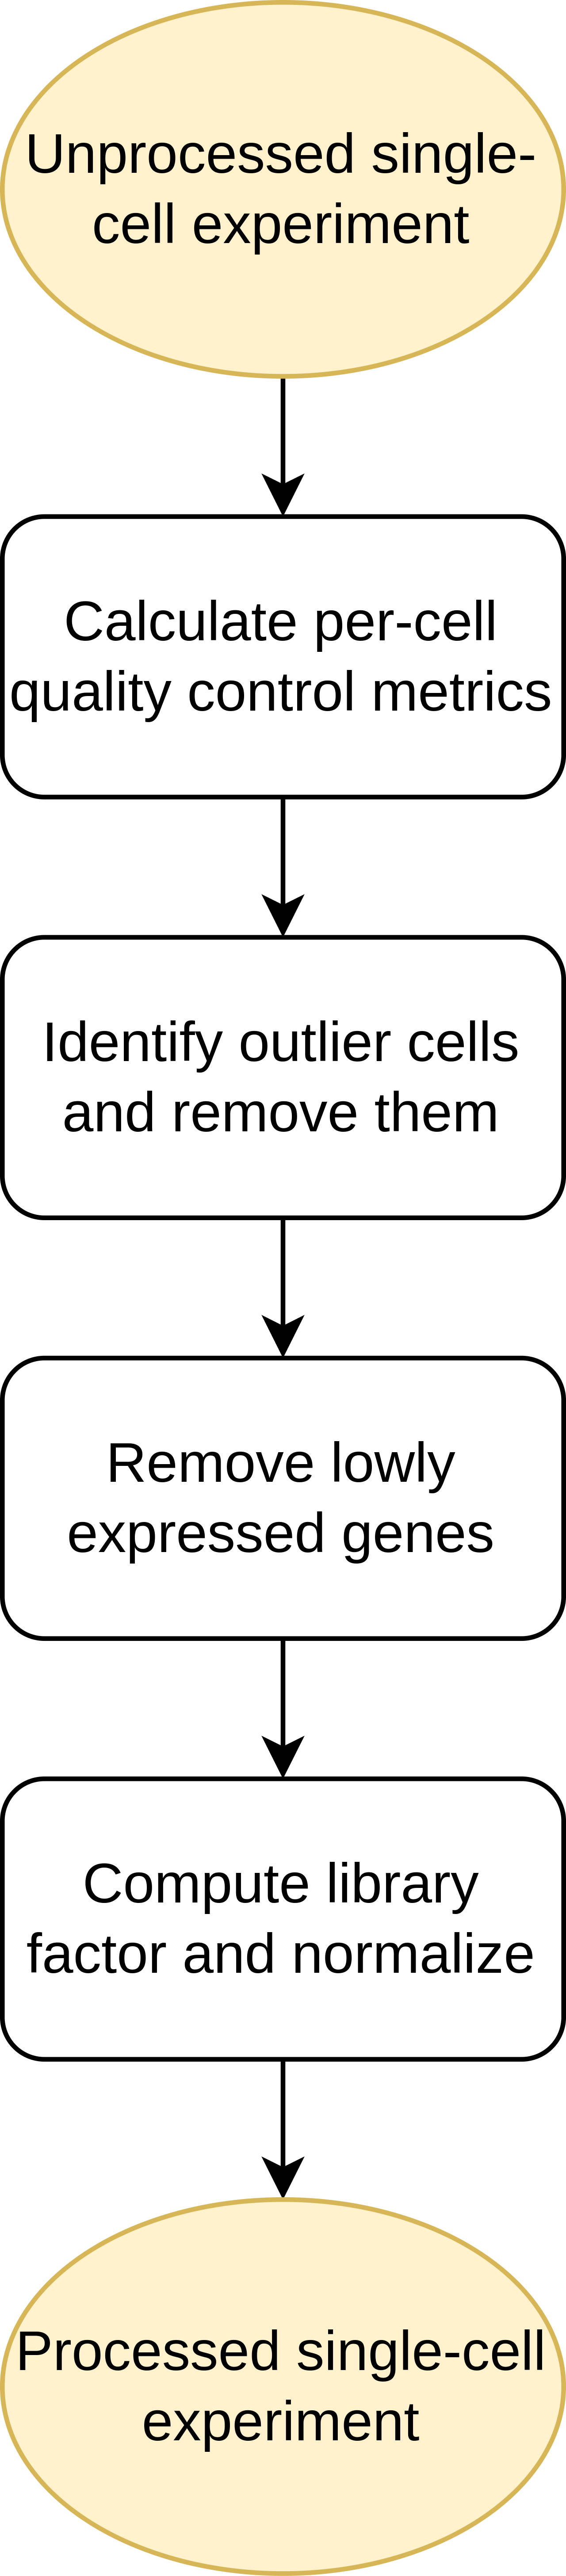
\includegraphics[width=1.5in,height=5.5in]{../figures/qc.png}
\end{center}
\caption{Quality control process from unprocessed, raw to processed, filtered single-cell experiment}
\label{fig:QC}
\end{figure}

After filtering, the data set consists of 23'543 cells and 18'537 genes. Next, we used the \emph{singleR} function from the \emph{singleR} R package \citep{singleR} for cell-type annotation. Cell-type annotation is important to determine what biological state is represented by cell clusters which helps the interpretability of the results and their implications \citep{OSCA}. \emph{singleR} is a method that assigns labels based on the reference samples with the highest Spearman rank correlation while only using marker genes between pairs of labels to focus on the relevant differences between cell types \citep{singleR}. Figure \ref{fig:UMAP_mouse_sample_id} shows the UMAP of the cells coloured by their respective sample id. From Figure \ref{fig:UMAP_mouse_sample_id} one can observe that the projection of the cells is very similar across the samples. Further, Figure \ref{fig:UMAP_mouse_cell_type} also illustrates that cells from the same cell-type cluster together, as one would expect.

Figure \ref{fig:mouse_cell_type} shows that the annotated cells were largely classified as either: Adipocytes, Epithelial cells and Hepatocytes. Additionally, one can observe that those three cell types are approximately evenly distributed across the four samples. For further analyses we focus on those cell types to investigate the performance of existing methods for the detection of differentially expressed genes and design our own simulation study.

\begin{figure}[!htb]
\begin{center}
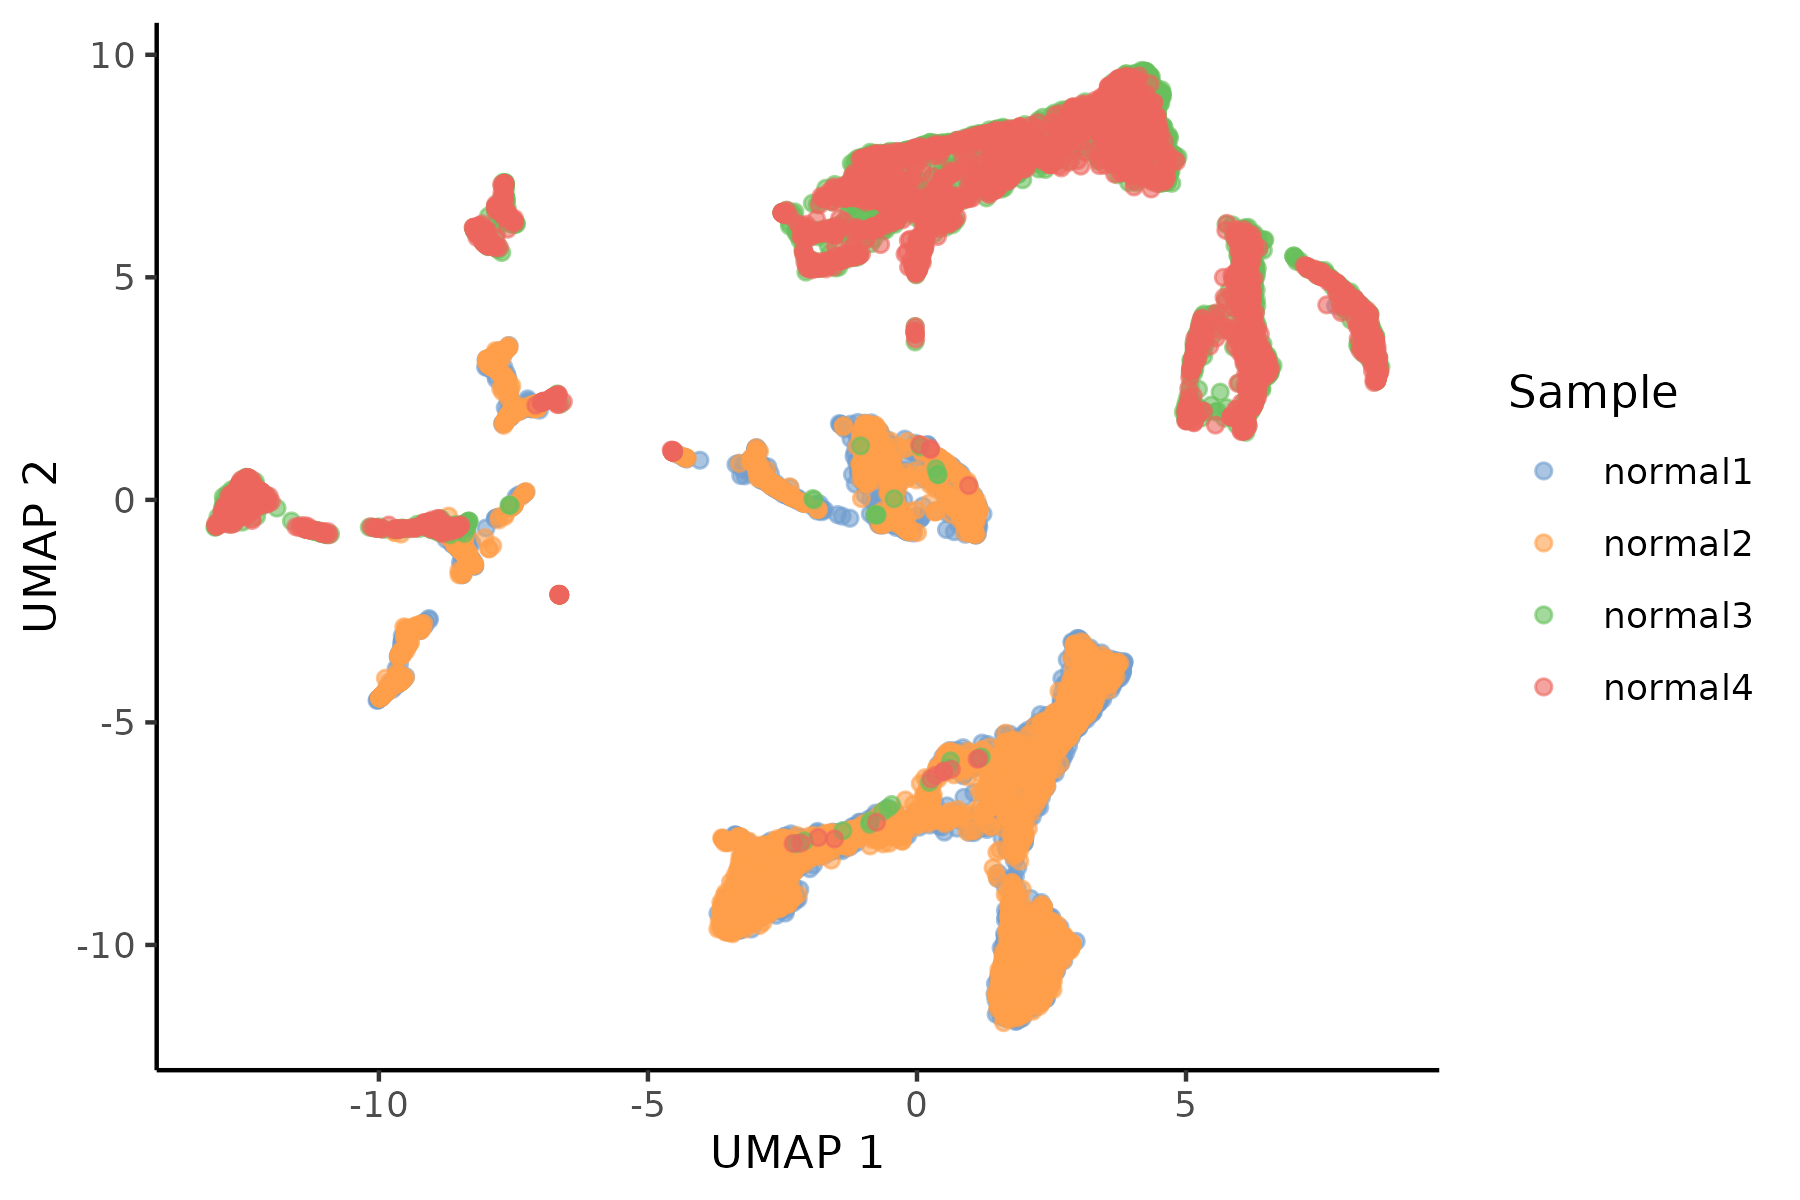
\includegraphics[width=6in,height=4in]{../figures/kidney_mouse/UMAP_mouse_sample_id.png}
\end{center}
\caption{UMAP representation of the mouse kidney cells coloured by sample id}
\label{fig:UMAP_mouse_sample_id}
\end{figure}

\begin{figure}[!htb]
\begin{center}
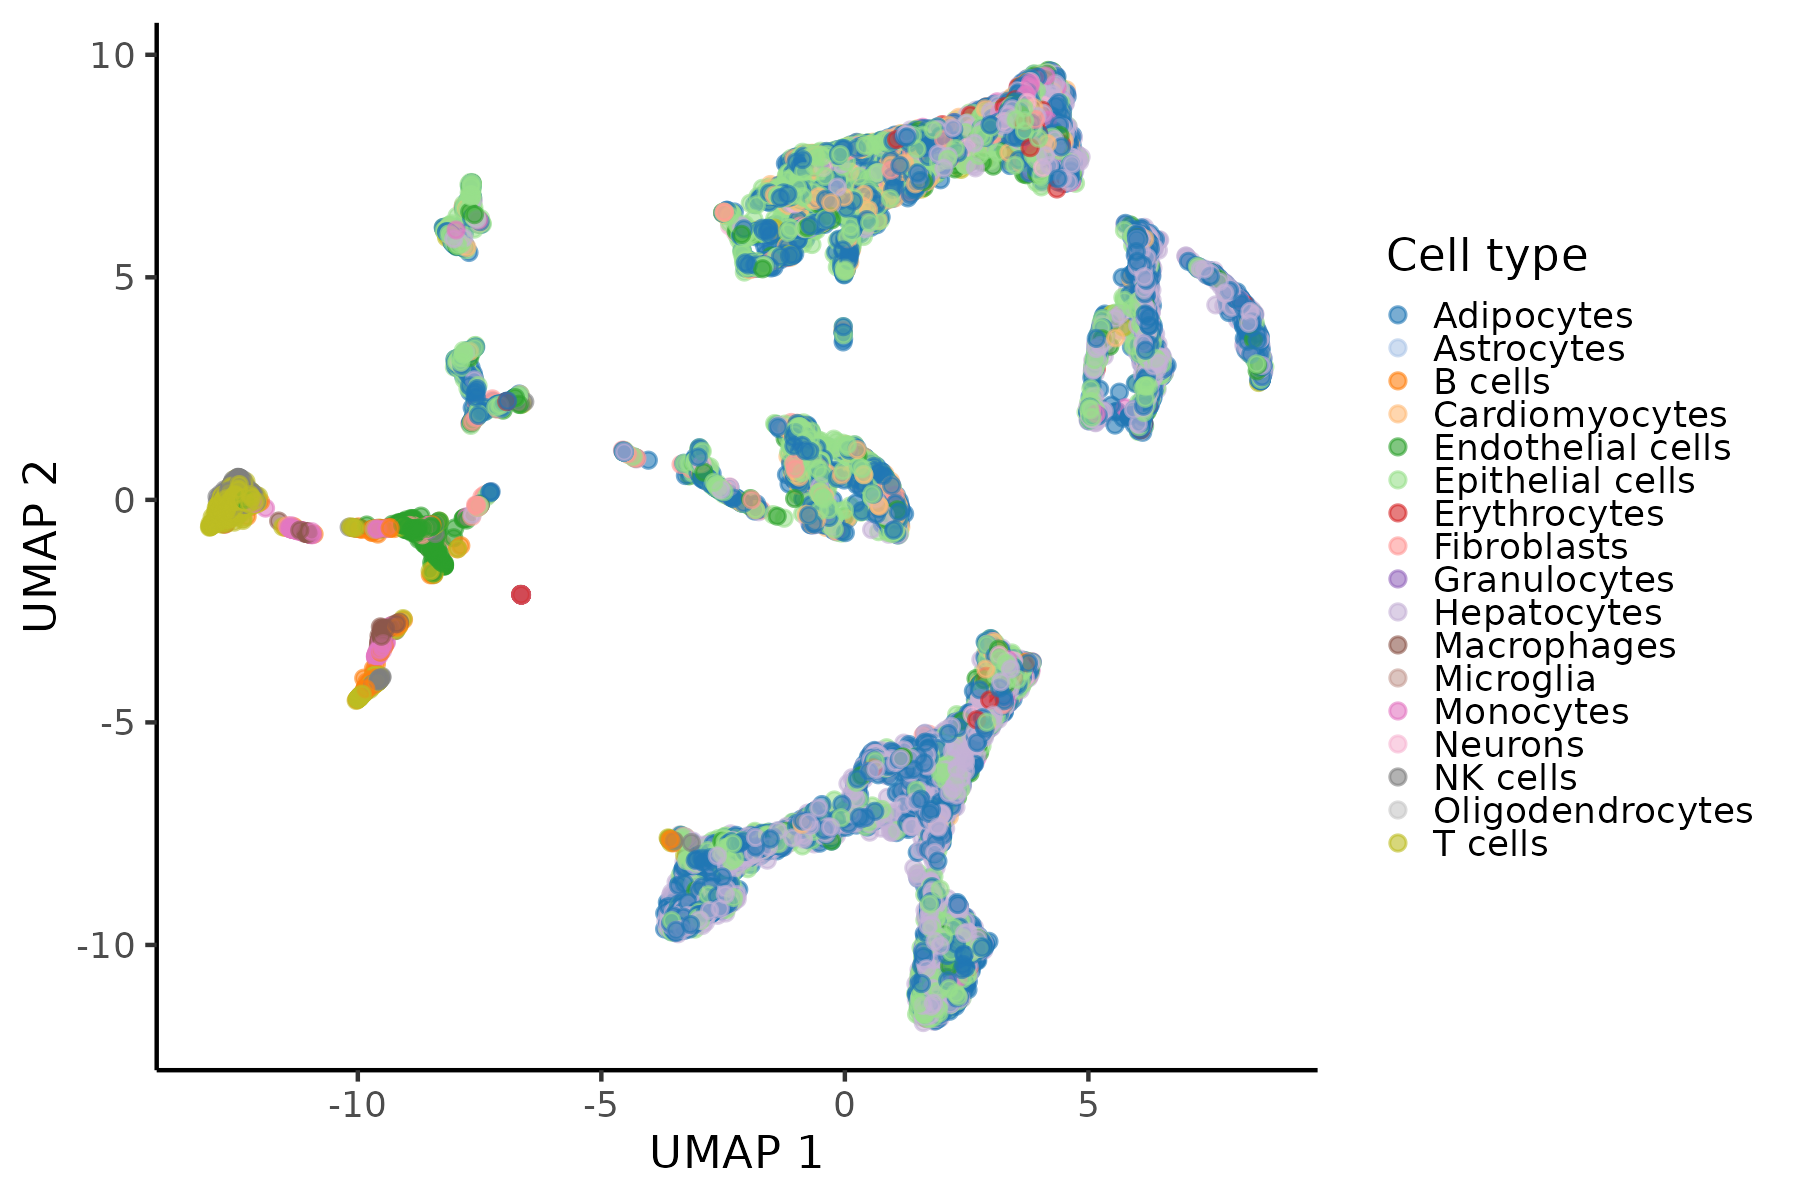
\includegraphics[width=6in,height=4in]{../figures/kidney_mouse/UMAP_mouse_cell_type.png}
\end{center}
\caption{UMAP representation of the mouse kidney cells coloured by cell type}
\label{fig:UMAP_mouse_cell_type}
\end{figure}

\begin{figure}[!htb]
\begin{center}
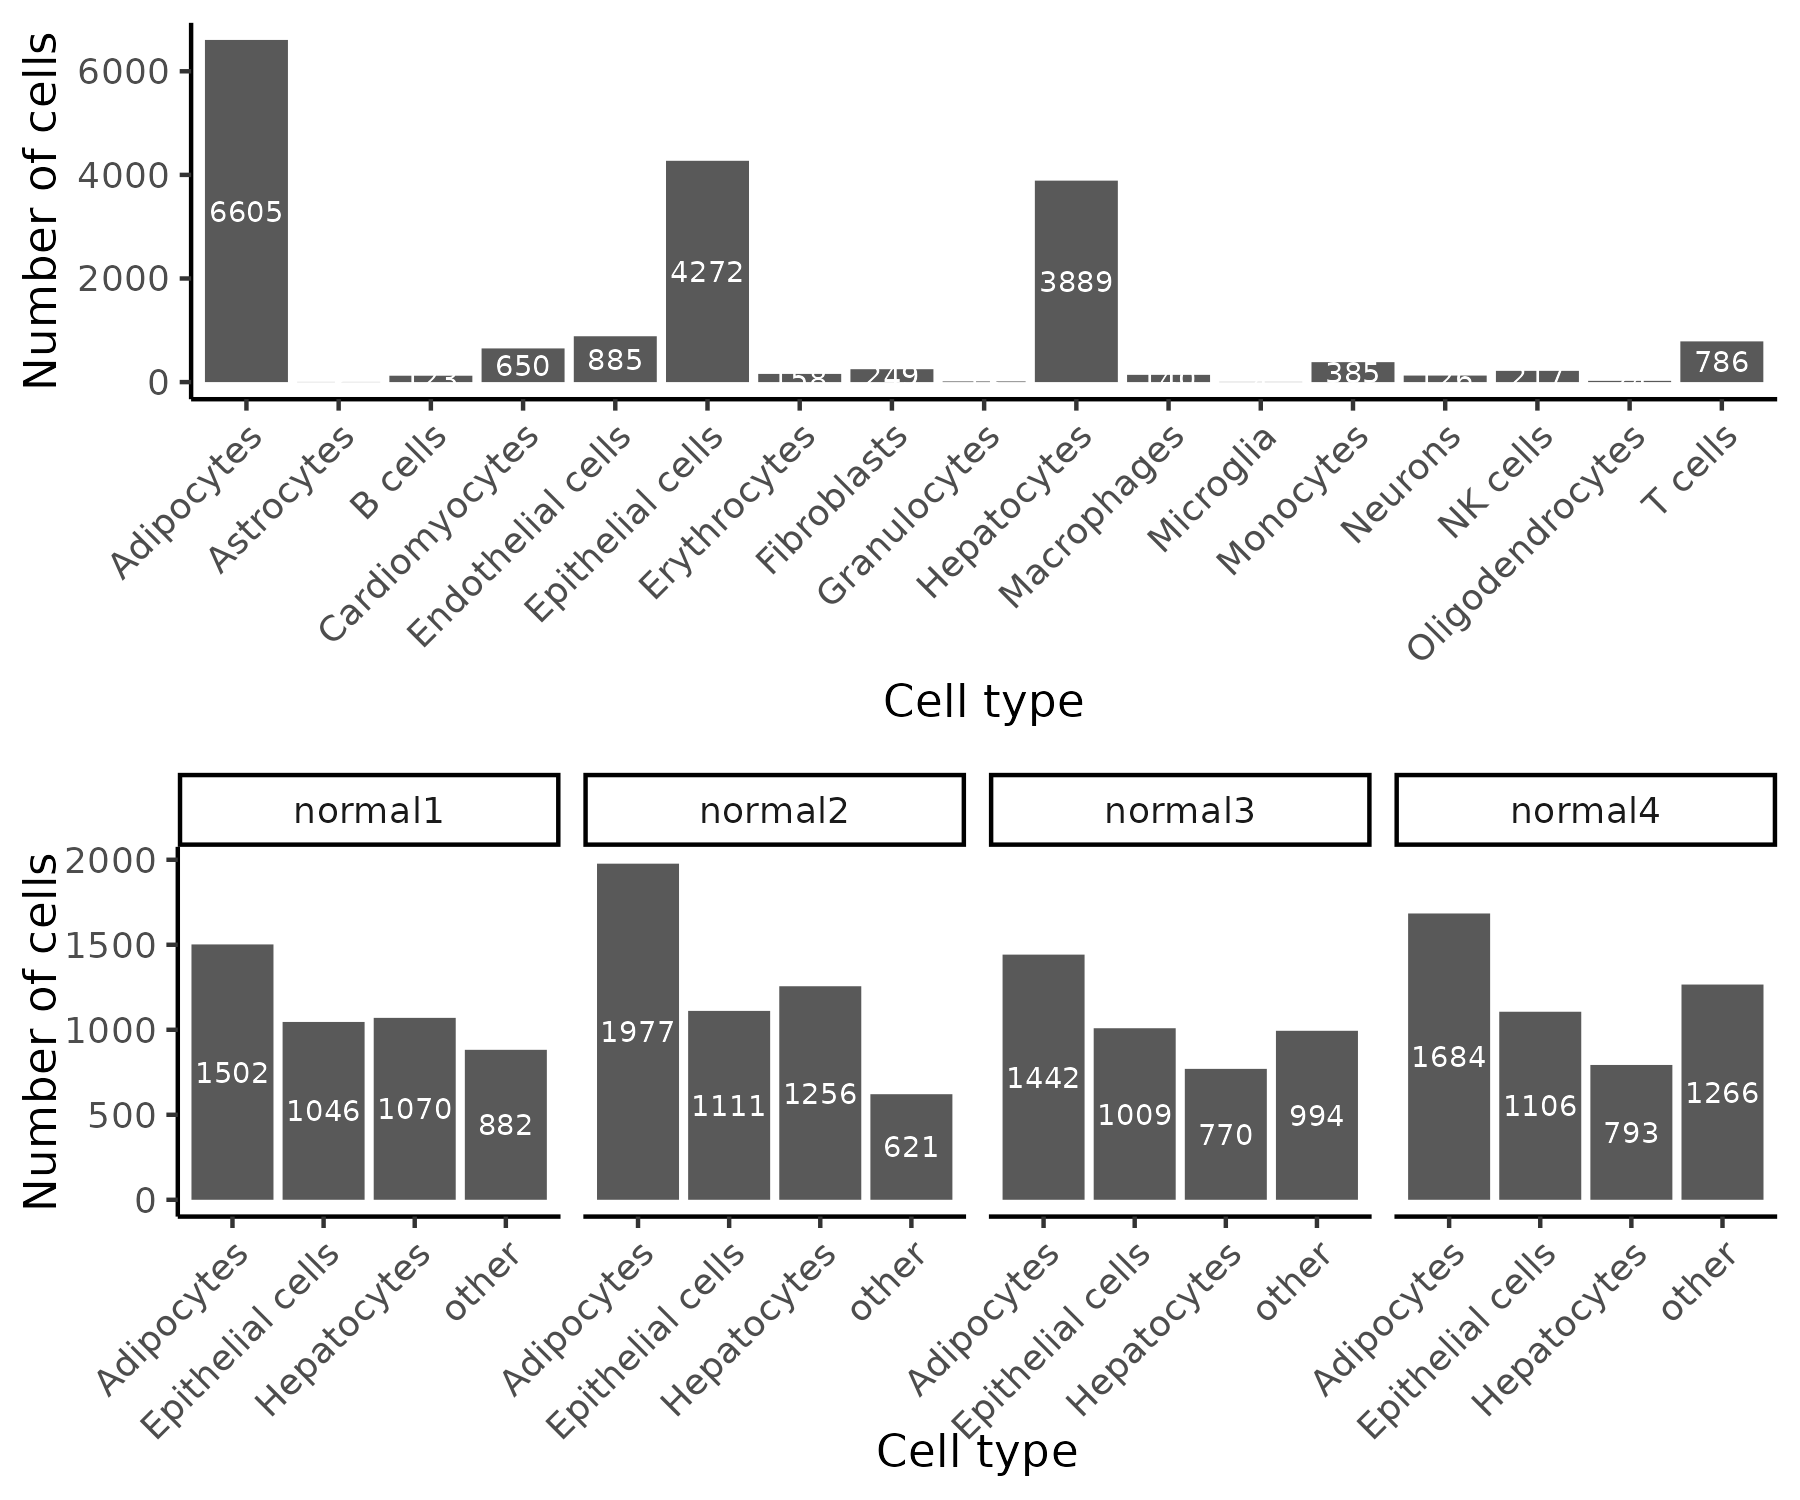
\includegraphics[width=6in,height=5in]{../figures/kidney_mouse/cell_type_distribution.png}
\end{center}
\caption{Frequency distribution of the cell types after quality control} 
\label{fig:mouse_cell_type}
\end{figure}

After QC filtering and cell type annotation we investigated the RNA velocities for each sample. Initially, we expected similar patterns with changing trajectories. First, we explored the proportions of spliced and unspliced counts in each sample. Figures \ref{fig:abundance_normal1} to \ref{fig:abundance_normal4} show that the abundance of spliced counts is very high in comparison to unspliced counts. In samples 3 and 4 the abundance of unspliced counts approximately half, compared to samples 1 and 2. After exploring the velocity plots there were no clear patterns that were consistent between the biological replicates as shown in Figures \ref{fig:velocity_normal1} to \ref{fig:velocity_normal4}. We initially thought that we could relate differentially regulated genes to differential velocity between experimental conditions. However, this does not seem possible. We therefore concluded that our discoveries (i.e. differences in the relative abundance of US or USA reads), cannot be taken as a proxy for "differential velocity". Although, the ideas of differential regulation and differential velocity are connected (i.e. RNA velocities are calculated on US estimated reads), we decided to keep the two concepts separate, and interpret our discoveries as differential regulated genes only.

\begin{figure}[!htb]
\begin{center}
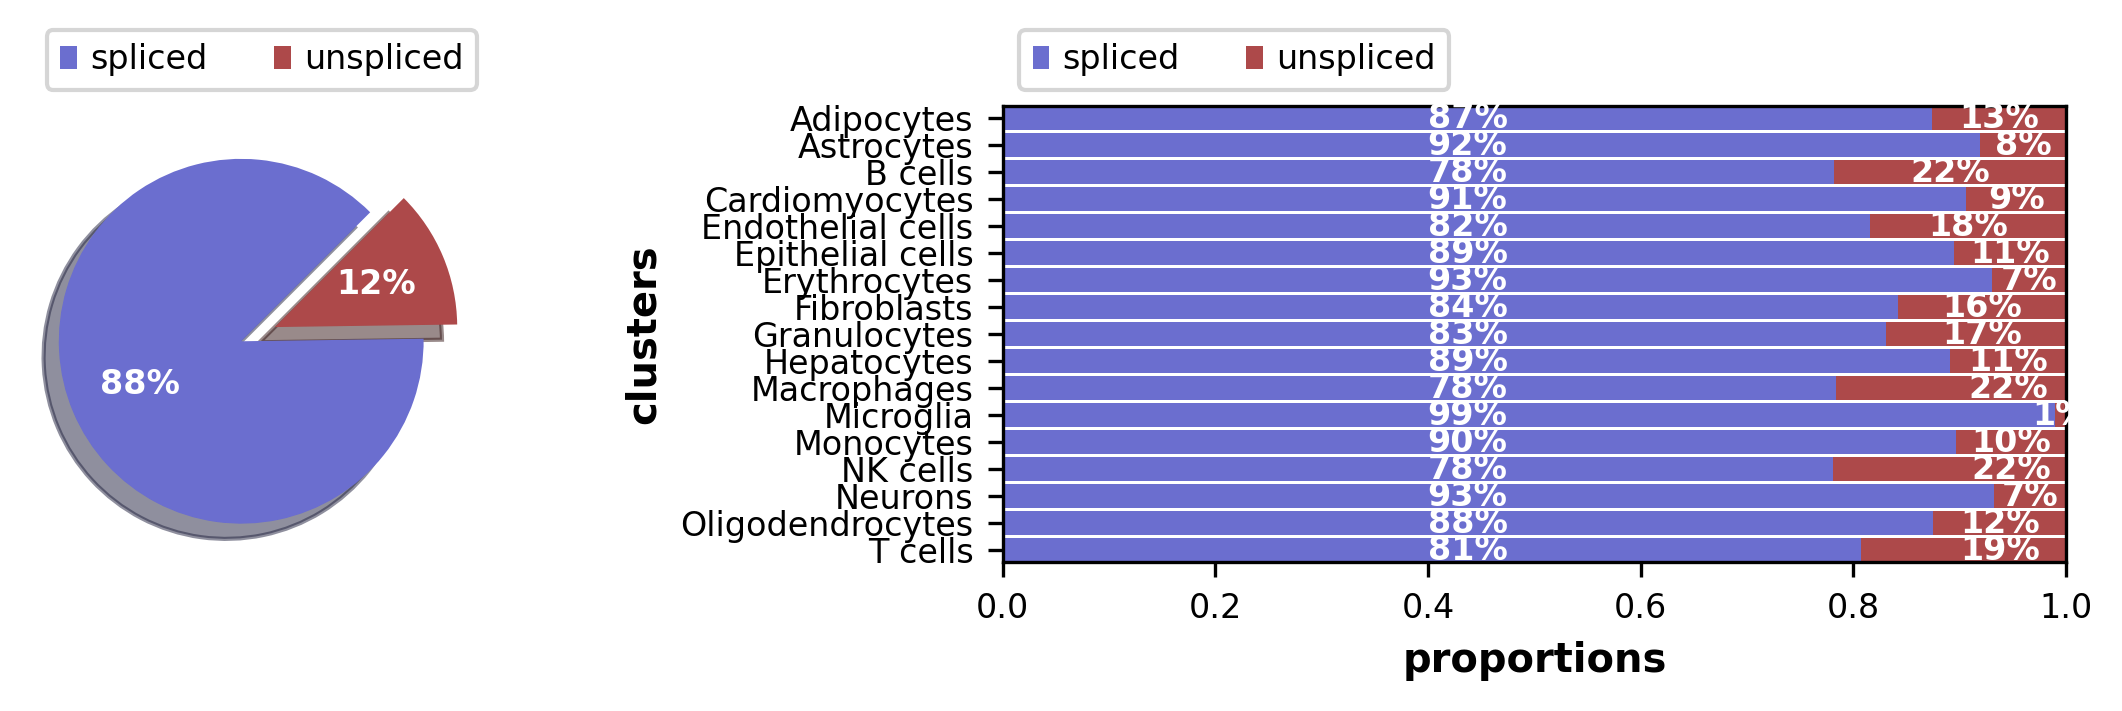
\includegraphics[width=6in,height=2in]{../figures/kidney_mouse/normal1_proportions.png}
\end{center}
\caption{Abundance of spliced and unspliced counts in sample normal1} 
\label{fig:abundance_normal1}
\end{figure}

\begin{figure}[!htb]
\begin{center}
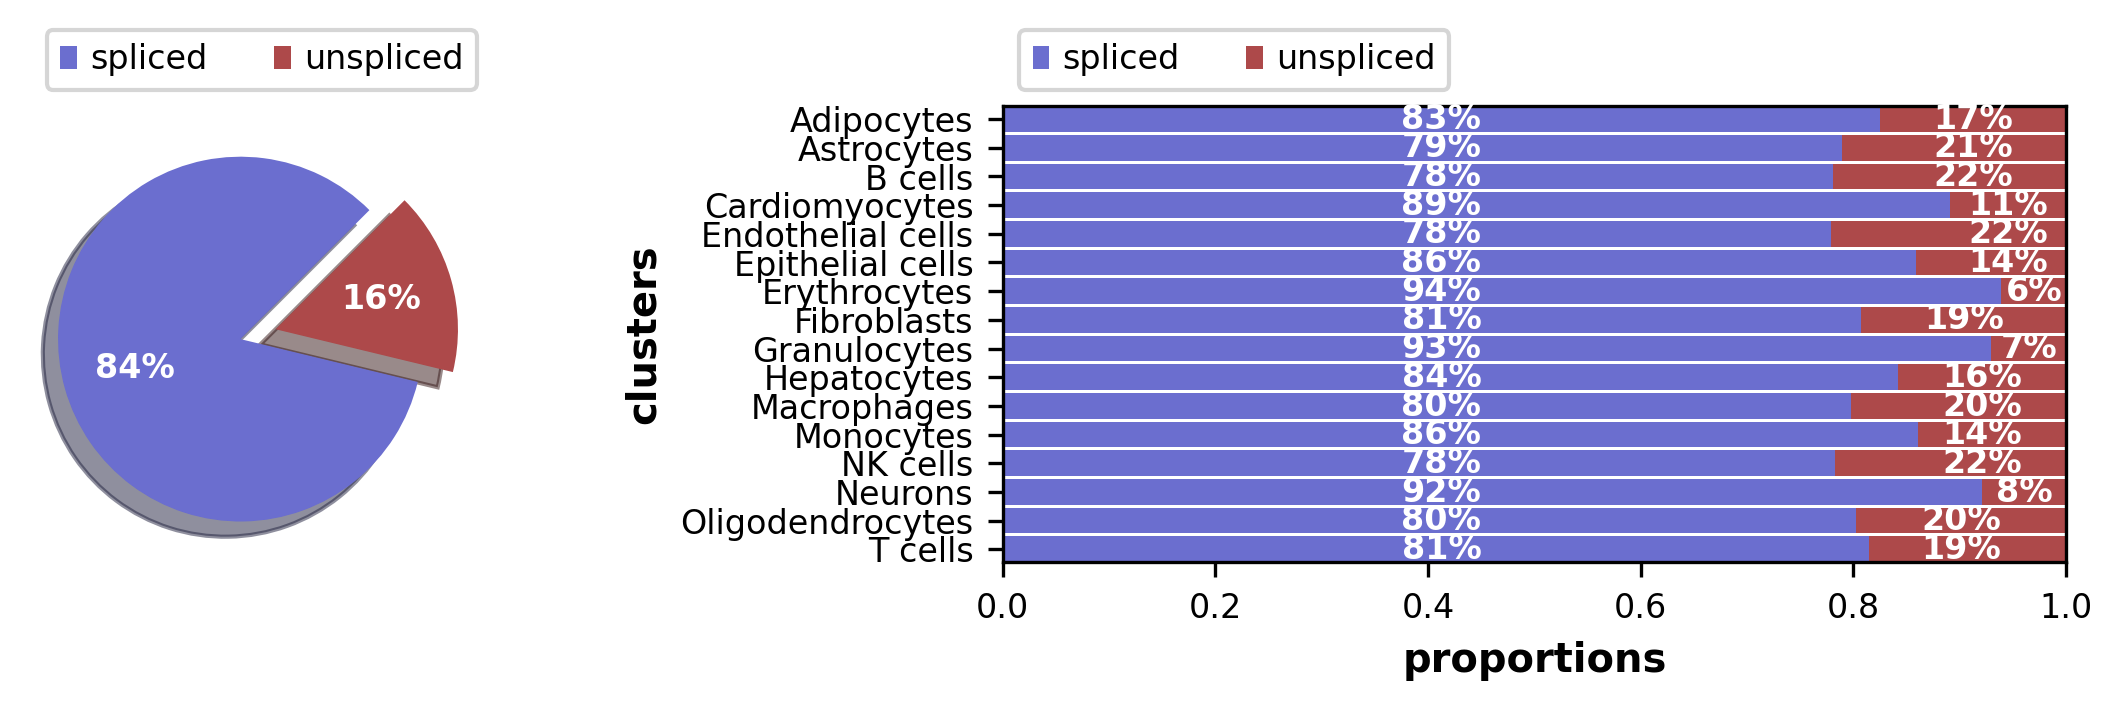
\includegraphics[width=6in,height=2in]{../figures/kidney_mouse/normal2_proportions.png}
\end{center}
\caption{Abundance of spliced and unspliced counts in sample normal2} 
\label{fig:abundance_normal2}
\end{figure}

\begin{figure}[!htb]
\begin{center}
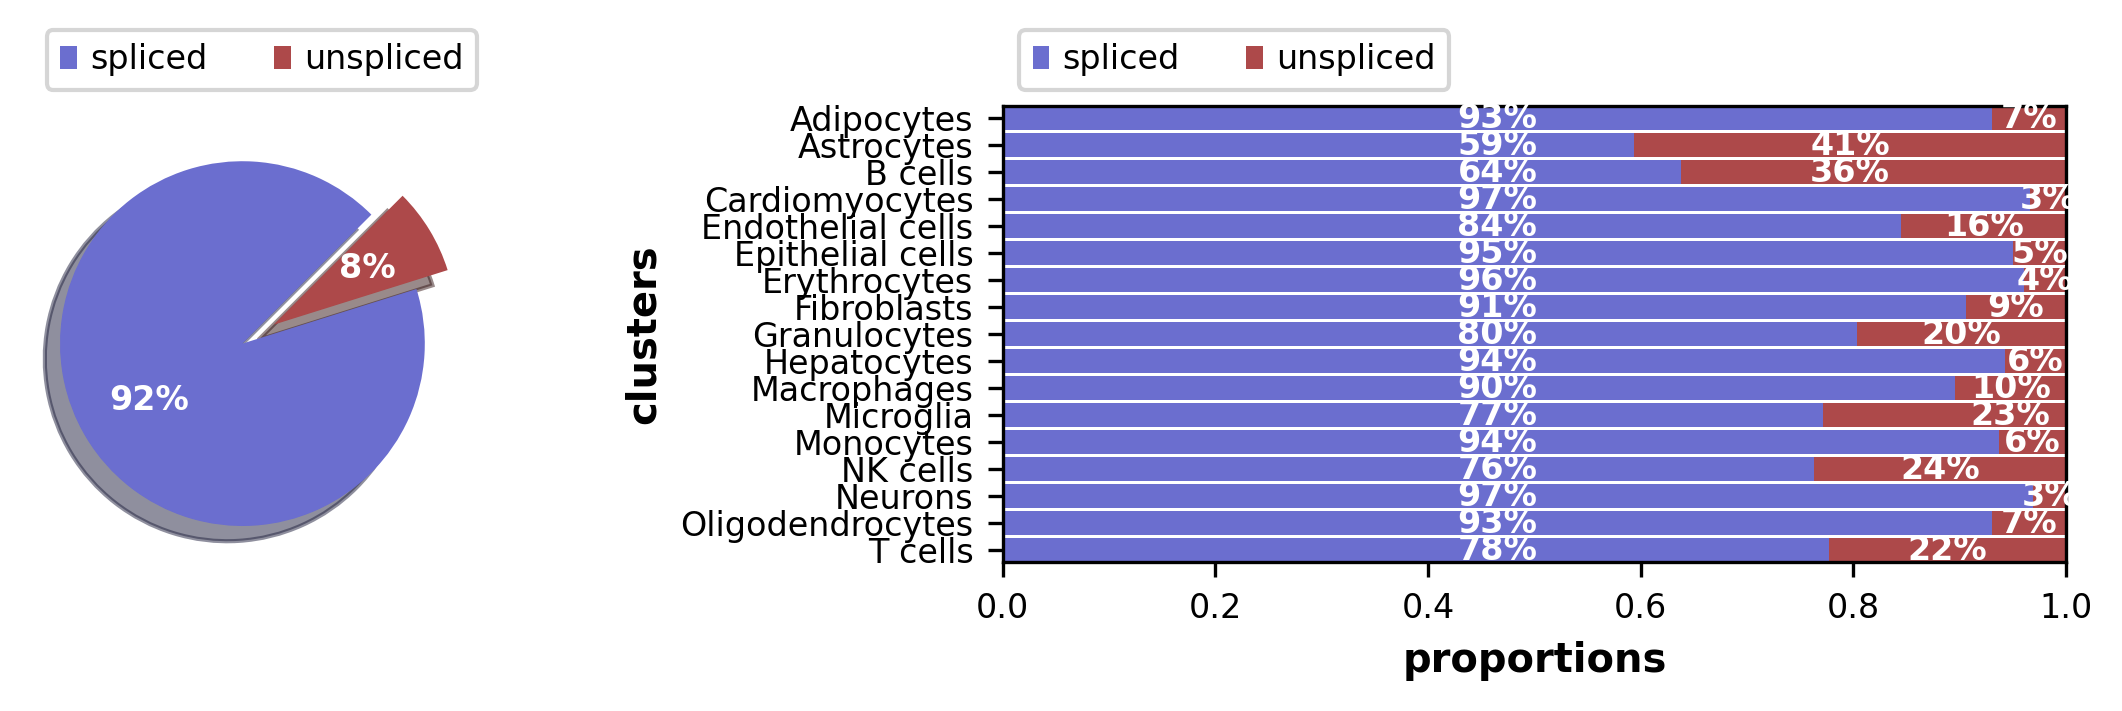
\includegraphics[width=6in,height=2in]{../figures/kidney_mouse/normal3_proportions.png}
\end{center}
\caption{Abundance of spliced and unspliced counts in sample normal3} 
\label{fig:abundance_normal3}
\end{figure}

\begin{figure}[!htb]
\begin{center}
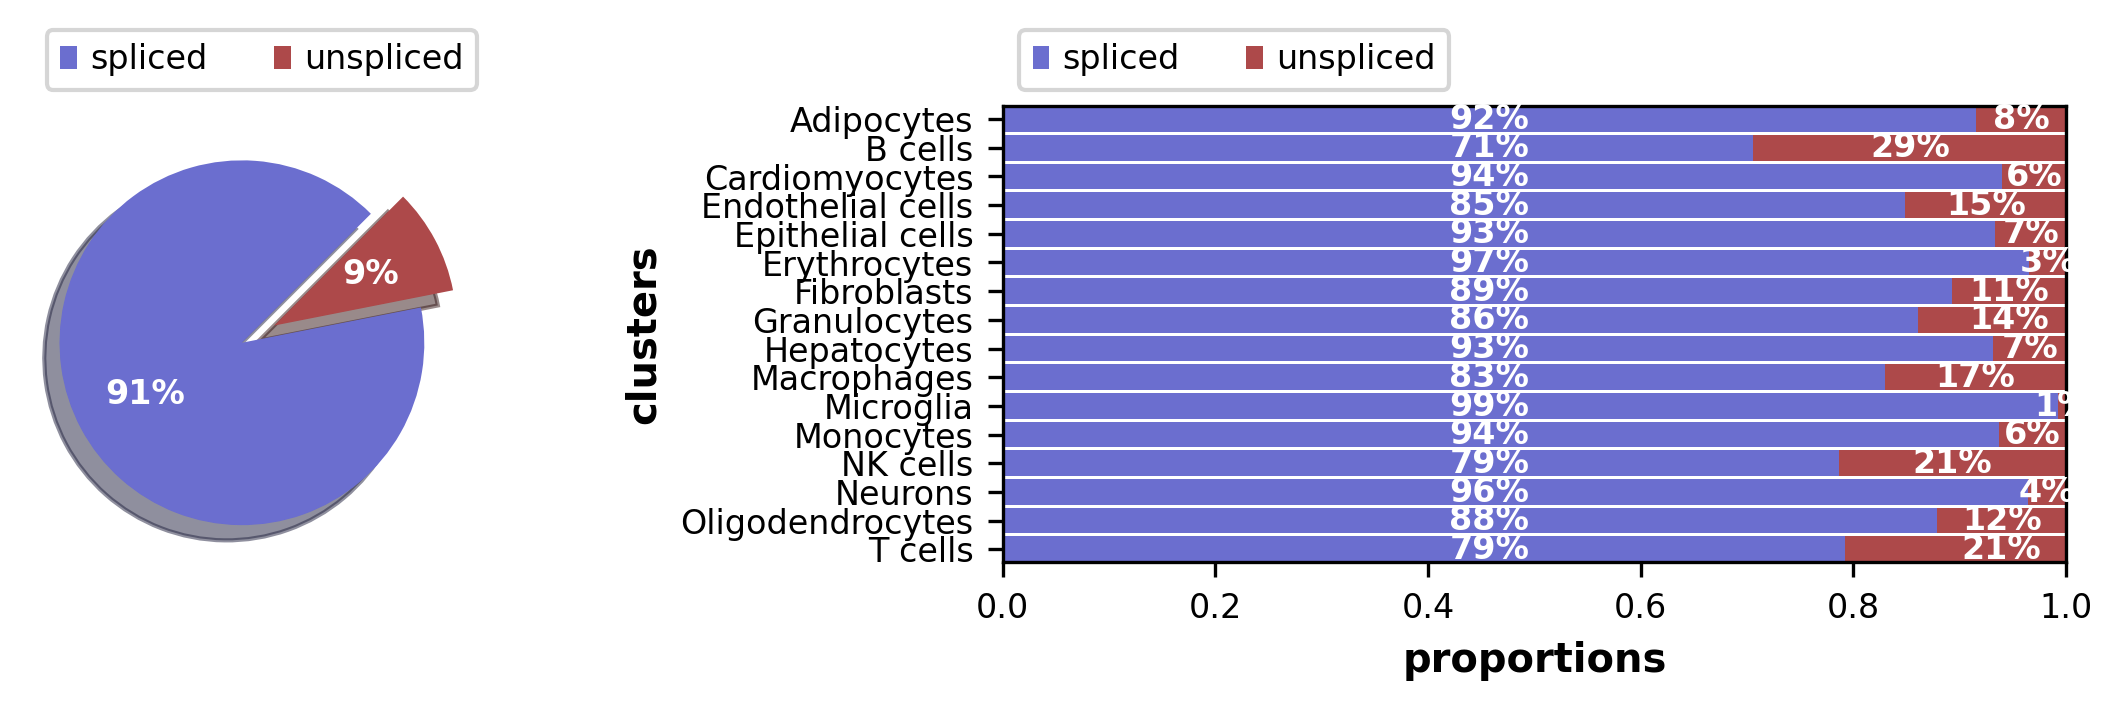
\includegraphics[width=6in,height=2in]{../figures/kidney_mouse/normal4_proportions.png}
\end{center}
\caption{Abundance of spliced and unspliced counts in sample normal4} 
\label{fig:abundance_normal4}
\end{figure}

\begin{figure}[!htb]
\begin{center}
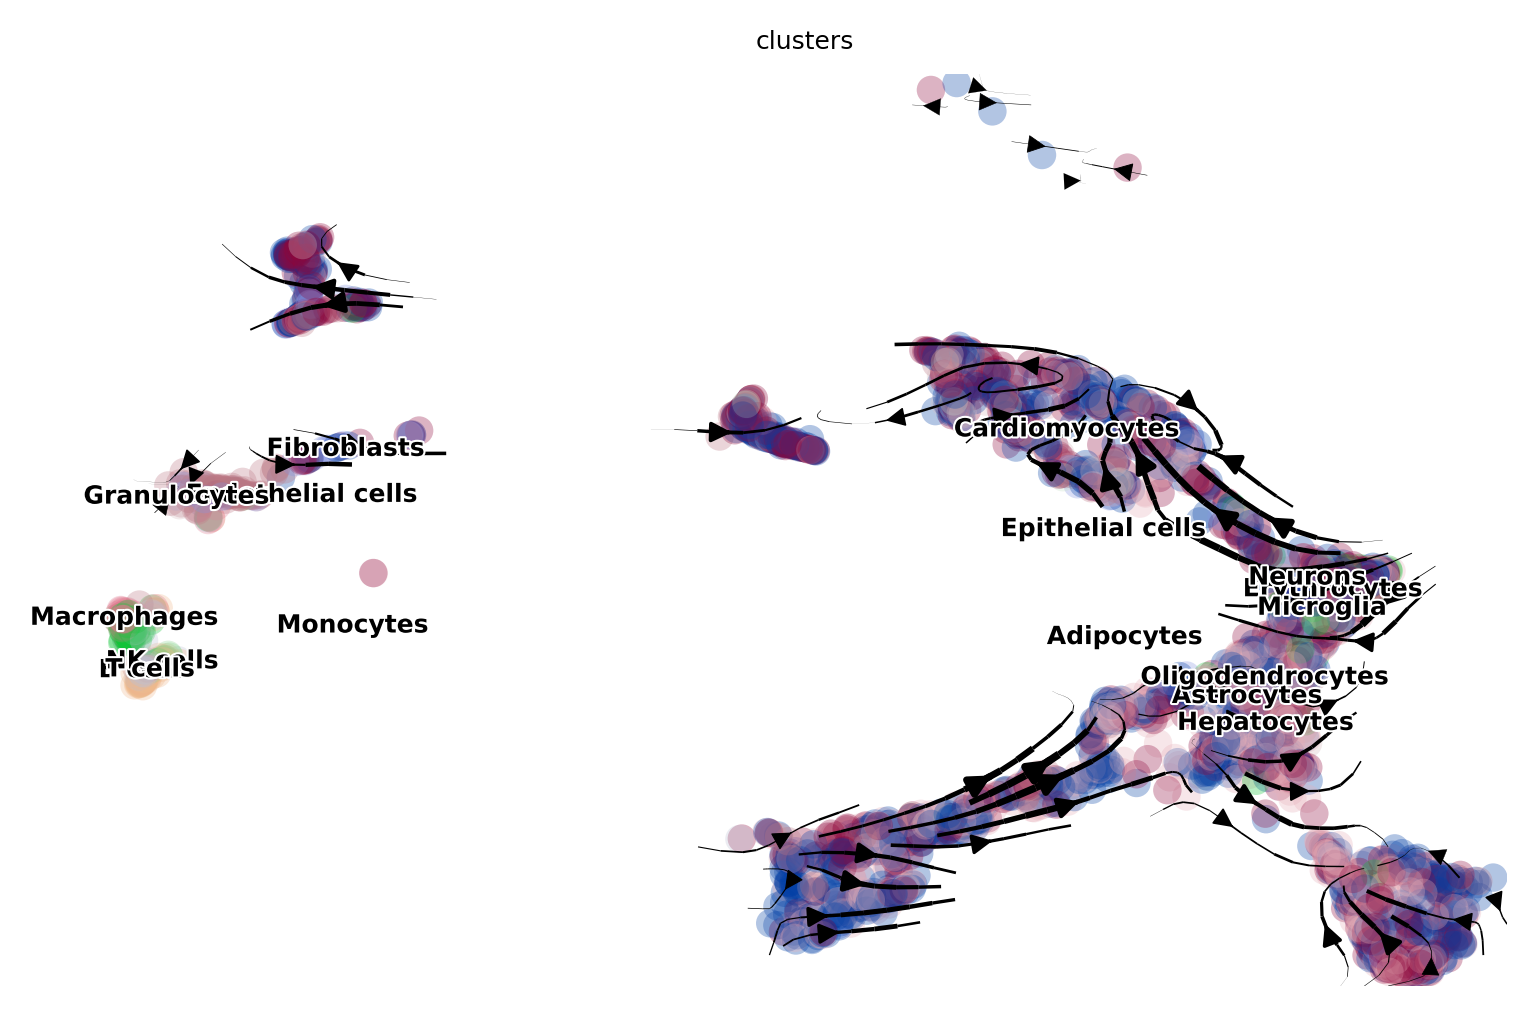
\includegraphics[width=6in,height=4in]{../figures/kidney_mouse/normal1_dynamical_model.png}
\end{center}
\caption{Dynamical model showing RNA velocity of sample normal1} 
\label{fig:velocity_normal1}
\end{figure}

\begin{figure}[!htb]
\begin{center}
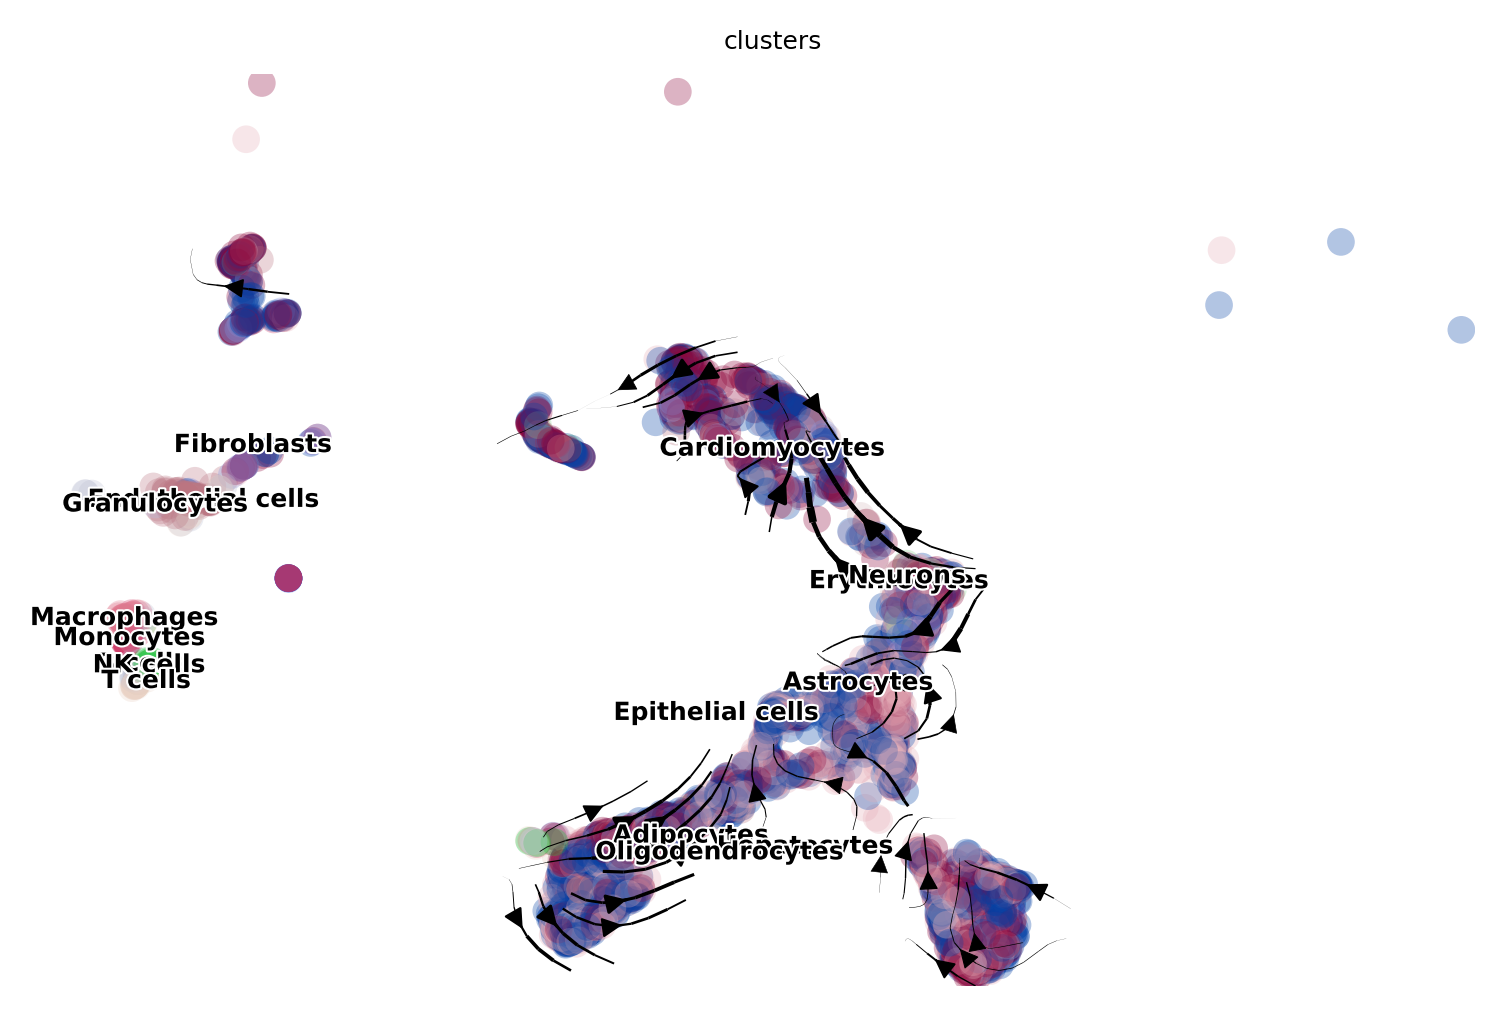
\includegraphics[width=6in,height=4in]{../figures/kidney_mouse/normal2_dynamical_model.png}
\end{center}
\caption{Dynamical model showing RNA velocity of sample normal2} 
\label{fig:velocity_normal2}
\end{figure}

\begin{figure}[!htb]
\begin{center}
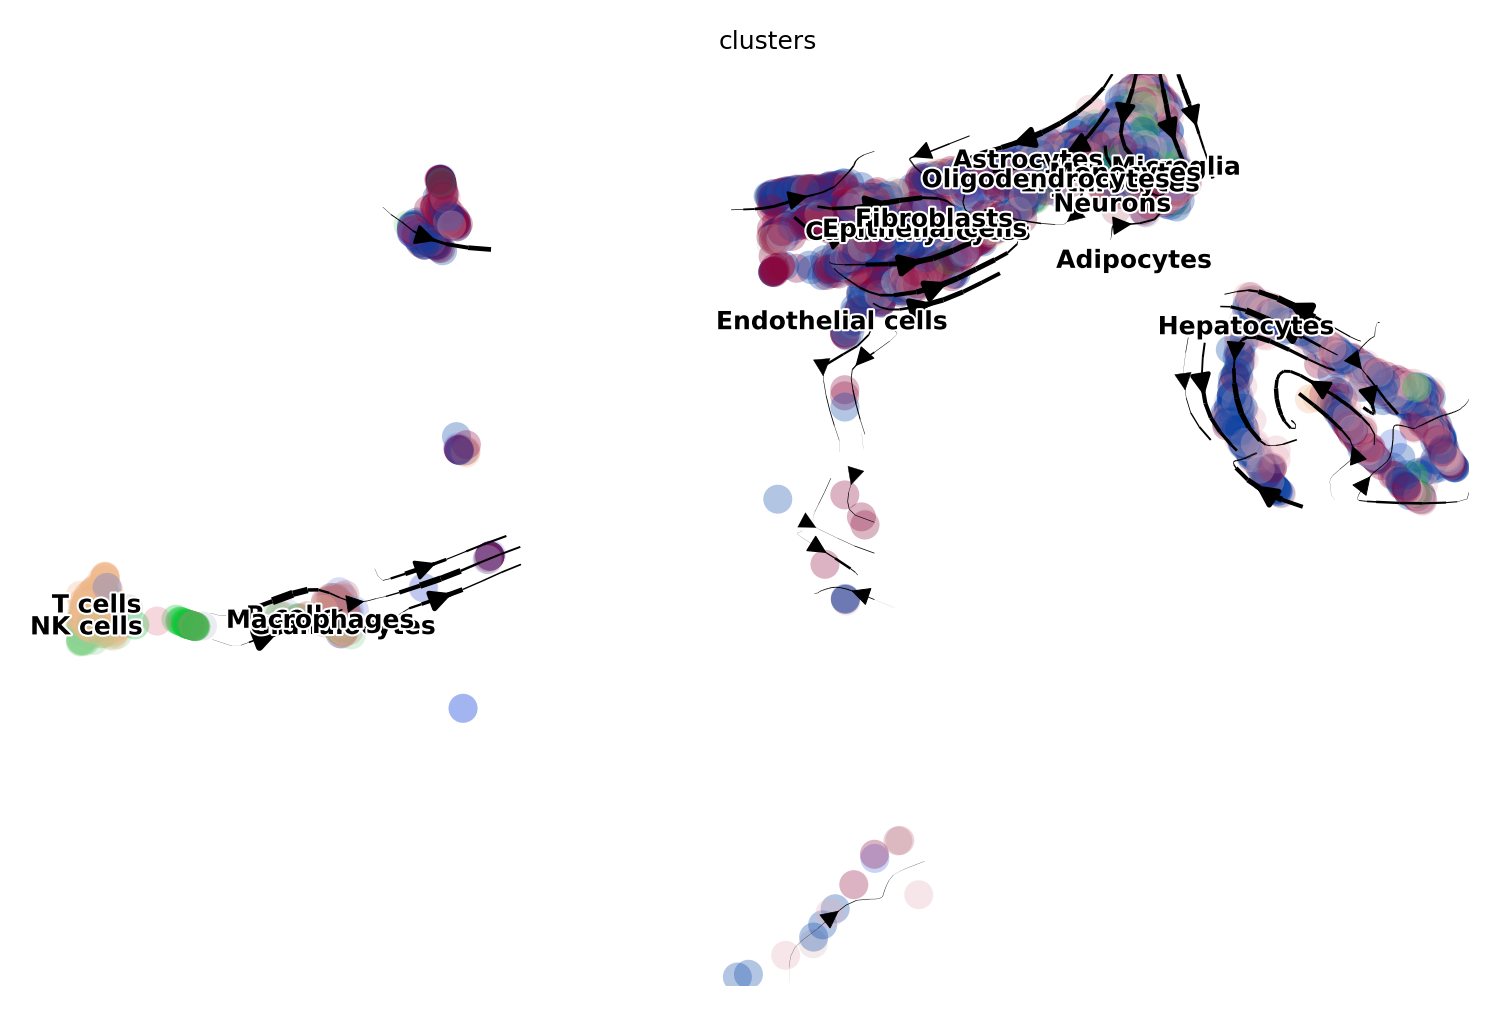
\includegraphics[width=6in,height=4in]{../figures/kidney_mouse/normal3_dynamical_model.png}
\end{center}
\caption{Dynamical model showing RNA velocity of sample normal3} 
\label{fig:velocity_normal3}
\end{figure}

\begin{figure}[!htb]
\begin{center}
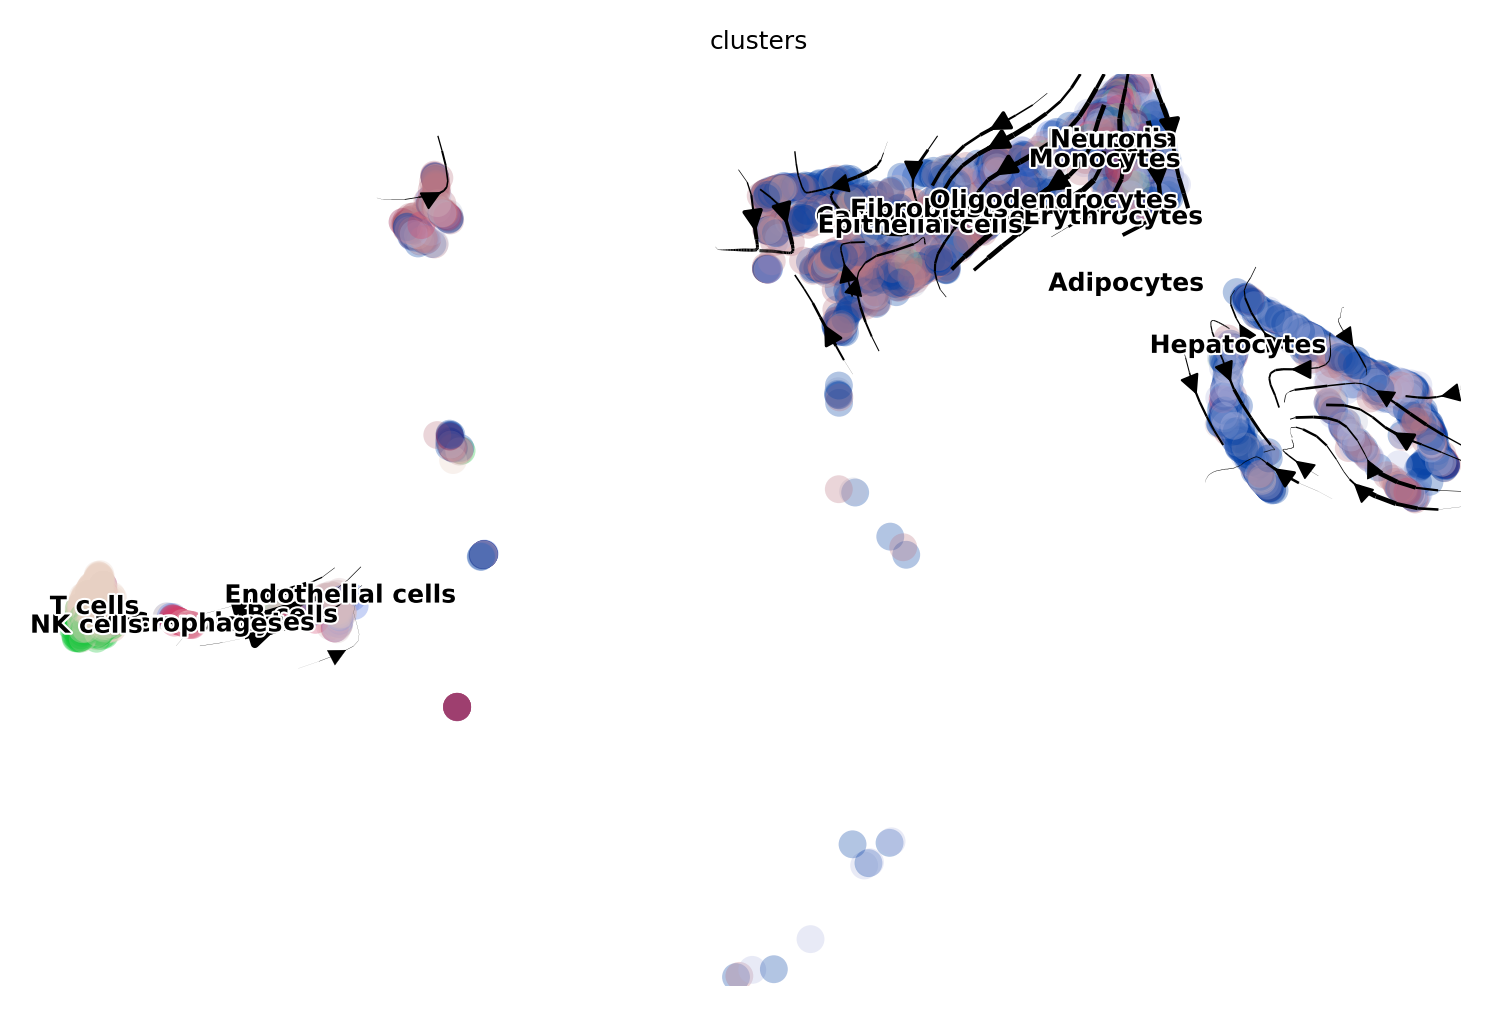
\includegraphics[width=6in,height=4in]{../figures/kidney_mouse/normal4_dynamical_model.png}
\end{center}
\caption{Dynamical model showing RNA velocity of sample normal4} 
\label{fig:velocity_normal4}
\end{figure}
\FloatBarrier

\section{Simulation study}

\subsection{Simulation strategy}
We designed two simulations: i) one where we simulated differentially regulated (DR) genes only and ii) one where we simulated both DR and differentially gene expression (DGE). In the second simulation, DGE was added as a nuisance effect that makes DR detection more challenging. Below, we first describe how to simulate DR effects, and then illustrate how DGE was added in the second simulation. Initially, the simulation strategy was to invert the spliced and unspliced counts for 10\% of genes for all cells that belong to an arbitrary group A. The group allocation was made based up on the consideration of the UMAP from Figure \ref{fig:UMAP_mouse_sample_id} where it is visible that samples tend cluster in pairs: 1 with 2, and 3 with 4. Therefore, the group allocation of $Group_A=(sample_1, sample_3)$ and $Group_B=(sample_2, sample_4)$ was chosen to obtain a homogeneous representation of the groups. The set of genes, whose counts were to be inverted, was randomly drawn by a sampling algorithm without replacement (hypergeometric distribution). There are many different ways to introduce a differential effect, however nailing down on inverting the spliced and unspliced counts seemed like a neat way to achieve this without actually modifying the originally estimated counts. This procedure was done separately for each cell type, so that differential genes are not the same across cell types. Additionally, in the second simulation only, DGE was introduced in 10\% of genes in all cells that belong to said arbitrary group A. In order to introduce DGE, we additionally multiply the counts by 10 (ten-fold gene expression) for 10\% randomly drawn genes in group A. Again, the set of genes was randomly drawn by the same sampling algorithm as before. 

Starting from a real data set as an anchor data set, then artificially introducing a differential effect, we essentially created two semi-simulated data sets. Compared to full simulations, semi-simulated approaches have the advantage of having a realistic structure, because it was indeed taken from real data. The genes and cells that were subject to change were stored as ground truth for further evaluation in the downstream analyses. Figure \ref{fig:simulation_process} illustrates the simulation process from the original mouse kidney data set to two simulated data sets.

\begin{figure}[!htb]
\begin{center}
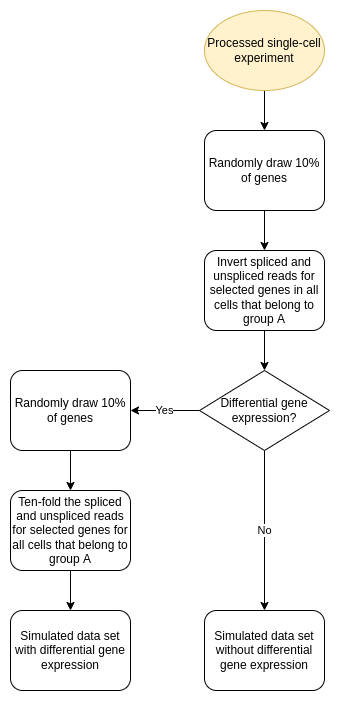
\includegraphics[width=3in,height=6in]{../figures/kidney_mouse/first_simulation_process.png}
\end{center}
\caption{Simulation process from original mouse data set to simulated data sets}
\label{fig:simulation_process}
\end{figure}

The goal of this thesis was to determine how well the aforementioned methods perform on detecting differentially regulated genes on read-level simulated data sets and the effect  of multi-mapping uncertainty. To achieve this two groups of methods were postulated as \emph{eisaR} and \emph{BRIE2} cannot take into account ambiguous reads. For this reason the classification performance of \emph{eisaR} and \emph{BRIE2} are compared with each other with the help of ROC and TPR v. FDR curves. As \emph{alevin-fry} allows the estimation of ambiguous counts as well as spliced and unspliced, it was possible to assign the ambiguous counts to both spliced and unspliced counts (50-50 split) so that \emph{eisaR} and \emph{BRIE2} can be applied. We settled to assign 50\% of ambiguous count to spliced and the other 50\% to unspliced because other methods, such as \emph{alevin}, also use this approach. In a similar manner, \emph{DEXSeq} and our own method \emph{DifferentialRegulation} were used to detect differentially regulated genes. However, in this case the ambiguous counts were used as an additional information. As a next step, \emph{minnow} was used to introduce mapping uncertainty into the simulated data sets. The simulated matrix of US counts was provided to \emph{minnow} to simulate scRNA-seq data at the read-level, which was then aligned and quantified with \emph{alevin-fry}. In order to assess the impact of multi-mapping uncertainty, we fit \emph{eisaR} and \emph{BRIE2} (the only methods that require US counts), to the original US simulated matrix (i.e. the input of \emph{minnow}), and to the US counts estimated from \emph{alevin-fry} (after running \emph{minnow}). The two analyses are shown in the next two sections, \ref{naive_sim} and \ref{soph_sim}.

\subsection{Simulation without mapping uncertainty} \label{naive_sim}
As a first step, we looked at the results from the naive simulation for both data sets with and without DGE. Figures \ref{fig:naive_sim_ROC} and \ref{fig:naive_sim_FDR} show that both \emph{eisaR} and \emph{BRIE2} perform quite well in detecting differential genes. \emph{eisaR} has a slightly higher TPR as shown in the ROC curve. Although, both methods have a similar performance pattern in the ROC curve, the TPR v. FDR plot looks quite different between the two methods. From Figures \ref{fig:naive_sim_DGE_ROC} and \ref{fig:naive_sim_DGE_FDR} it is shown that \emph{eisaR} is well calibrated for FDR, whereas \emph{BRIE2} is not.

After introducing DGE in the second data set performance drops quite substantially as shown in Figure \ref{fig:naive_sim_DGE_ROC}. TPR is almost halved in both methods as it is shown in the ROC curve of Figure \ref{fig:naive_sim_DGE_ROC}. However, \emph{eisaR} is still well calibrated for FDR. Similar to the data set without DGE, \emph{BRIE2} is not well calibrated for FDR. It seems that both methods are heavily affected by the introduction of DGE as performance dropped to almost half. However, we introduced a very strong effect - 10 fold change - therefore, it is to be expected that performance drops. Nevertheless, we wanted to investigate how the performance changes in an extreme scenario, hence the strong effect size. 

From this naive simulation we concluded that \emph{BRIE2} has inflated FDR in both cases - with and without DGE. On the other hand, \emph{eisaR} was well calibrated for FDR in both cases. However, TPR decreases by almost half after introducing DGE. In th next step, we use \emph{minnow} to introduce multi-mapping uncertainty in to both data sets to make the simulation more realistic. It is to be expected that performance will further decrease after the introduction of multi-mapping uncertainty.

\begin{figure}[!htb]
\begin{center}
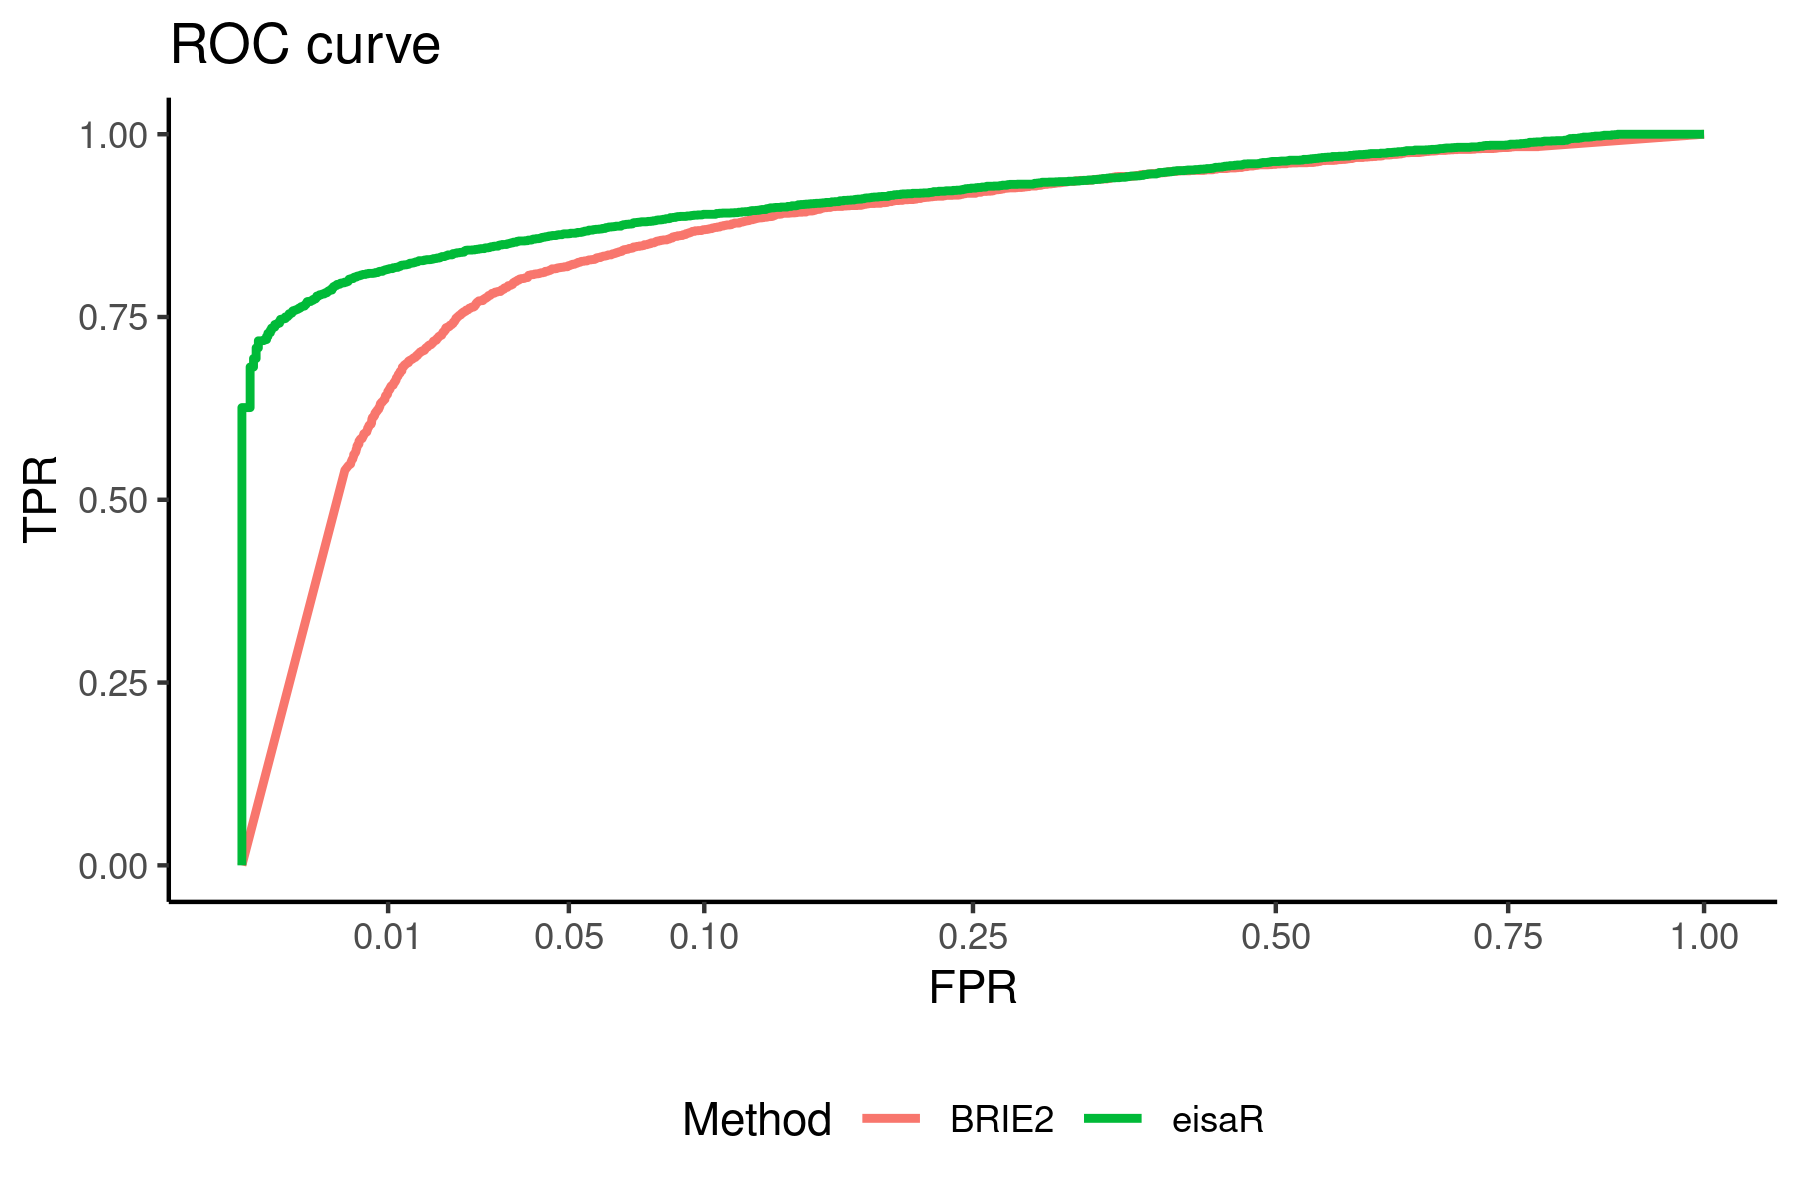
\includegraphics[width=6in,height=3.7in]{../figures/simulation/naive_simulation_ROC.png}
\end{center}
\caption{ROC curve of \emph{BRIE2} and \emph{eisaR} in the initial simulation without DGE}
\label{fig:naive_sim_ROC}
\end{figure}

\begin{figure}[!htb]
\begin{center}
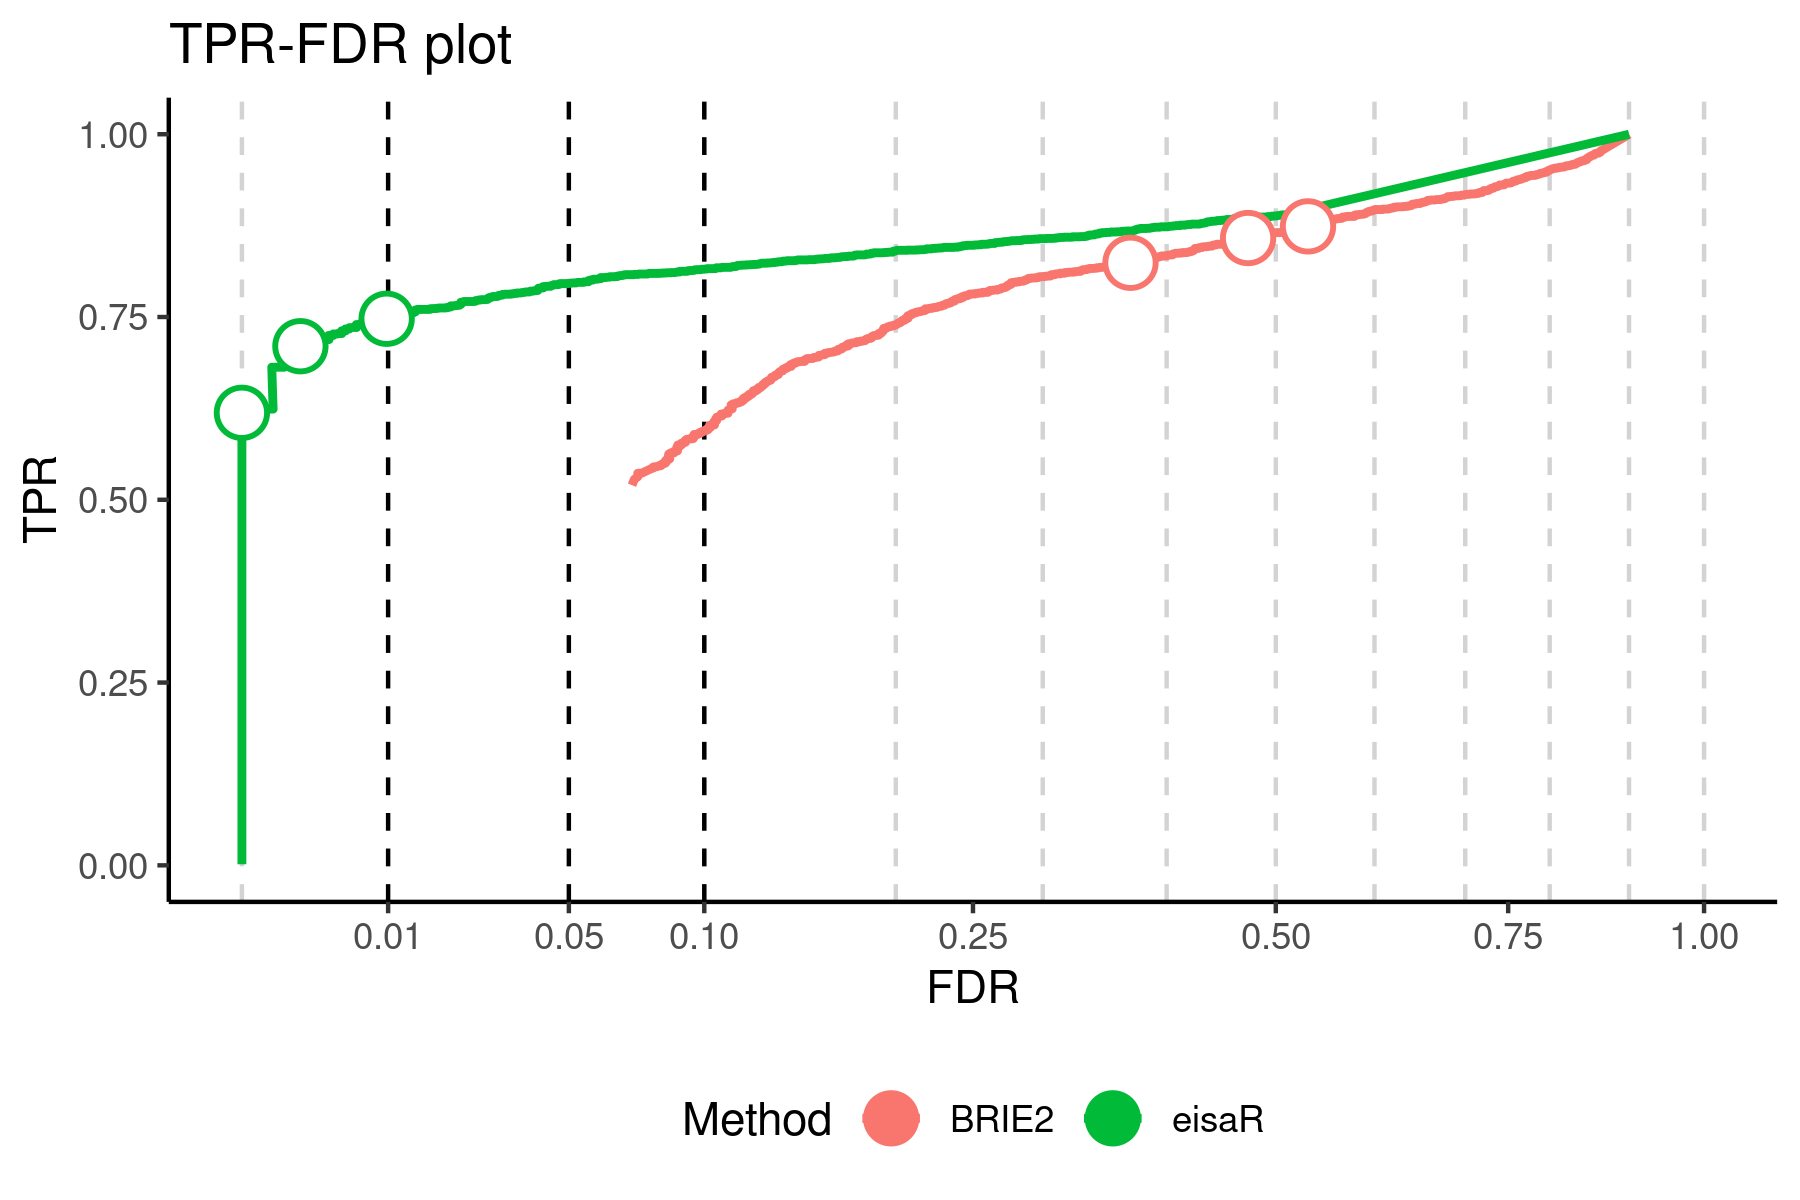
\includegraphics[width=6in,height=3.7in]{../figures/simulation/naive_simulation_FDR.png}
\end{center}
\caption{TPR v. FDR plot of \emph{BRIE2} and \emph{eisaR} in the initial simulation without DGE}
\label{fig:naive_sim_FDR}
\end{figure}

\begin{figure}[!htb]
\begin{center}
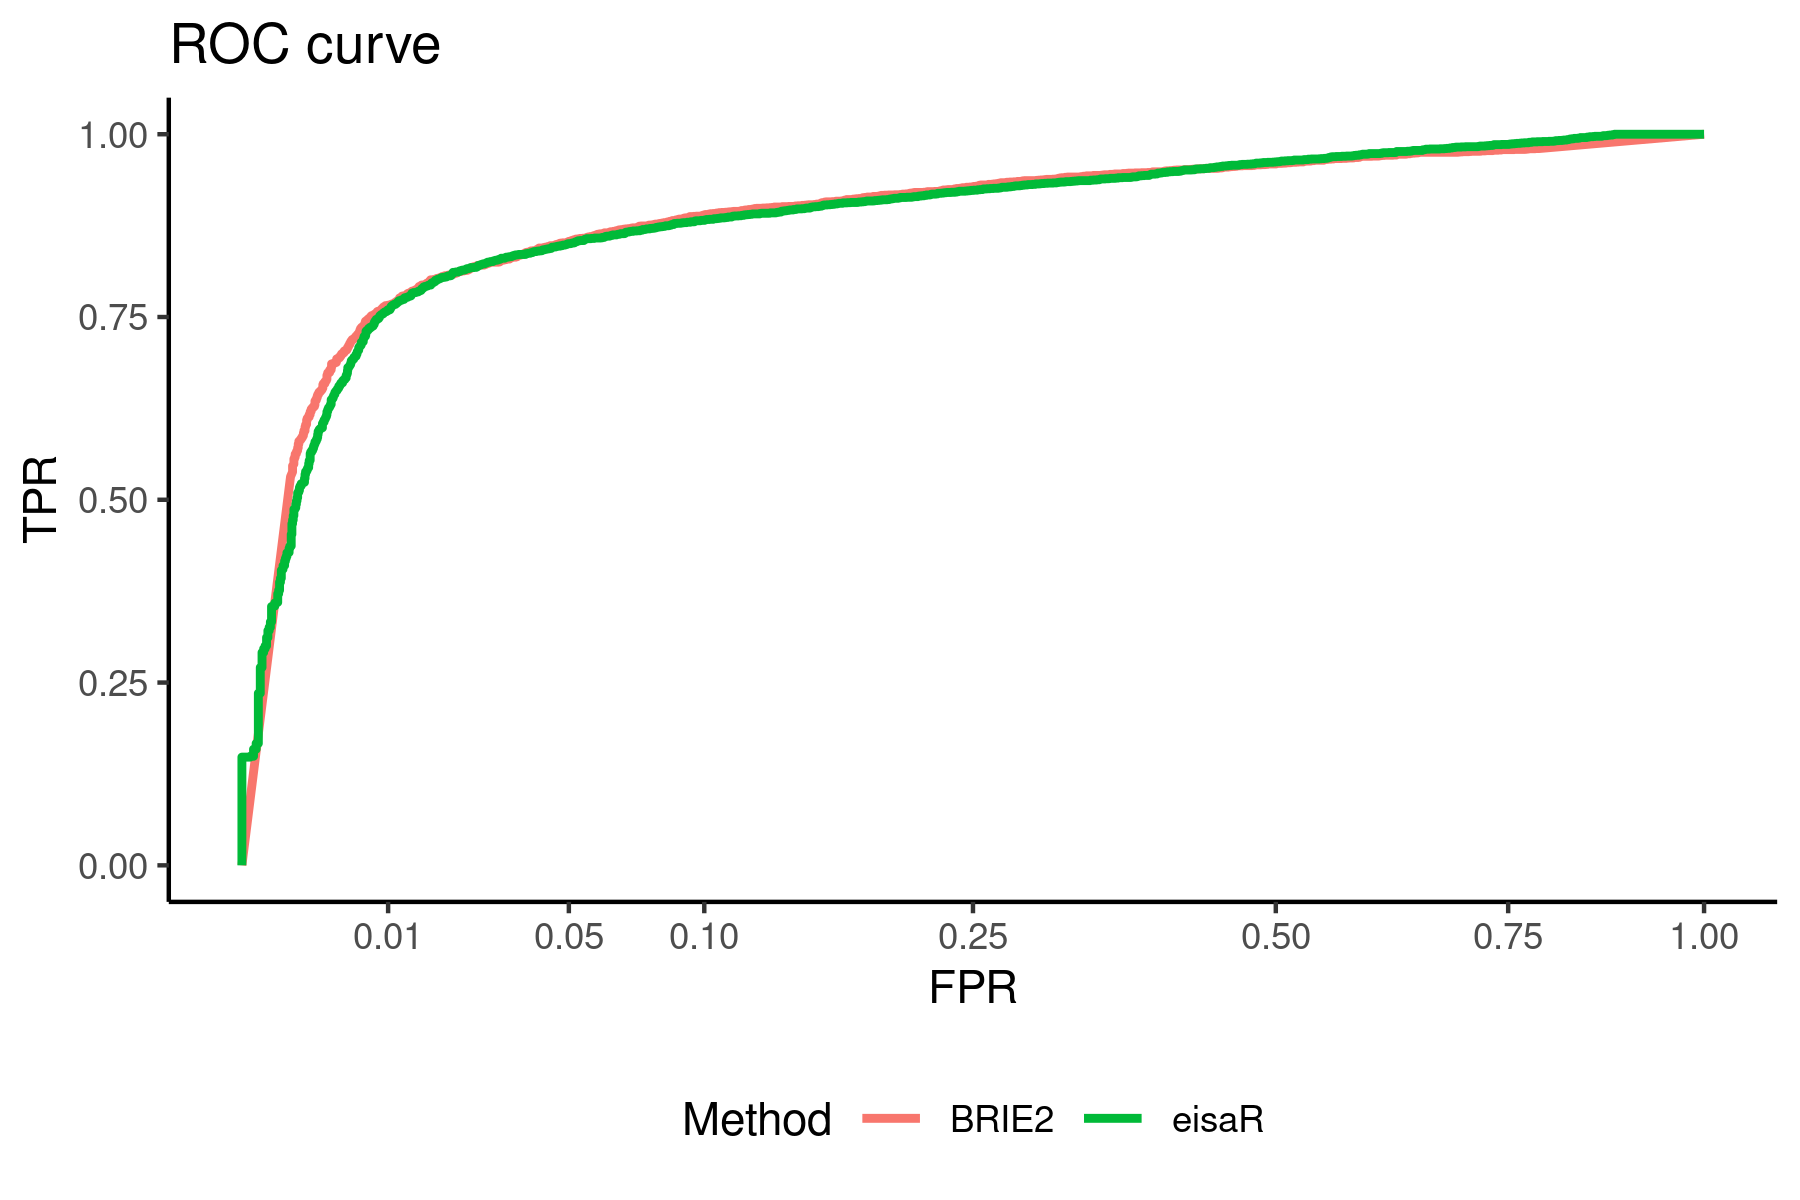
\includegraphics[width=6in,height=3.8in]{../figures/simulation/naive_simulation_DGE_ROC.png}
\end{center}
\caption{ROC curve of \emph{BRIE2} and \emph{eisaR} in the initial simulation with DGE}
\label{fig:naive_sim_DGE_ROC}
\end{figure}

\begin{figure}[!htb]
\begin{center}
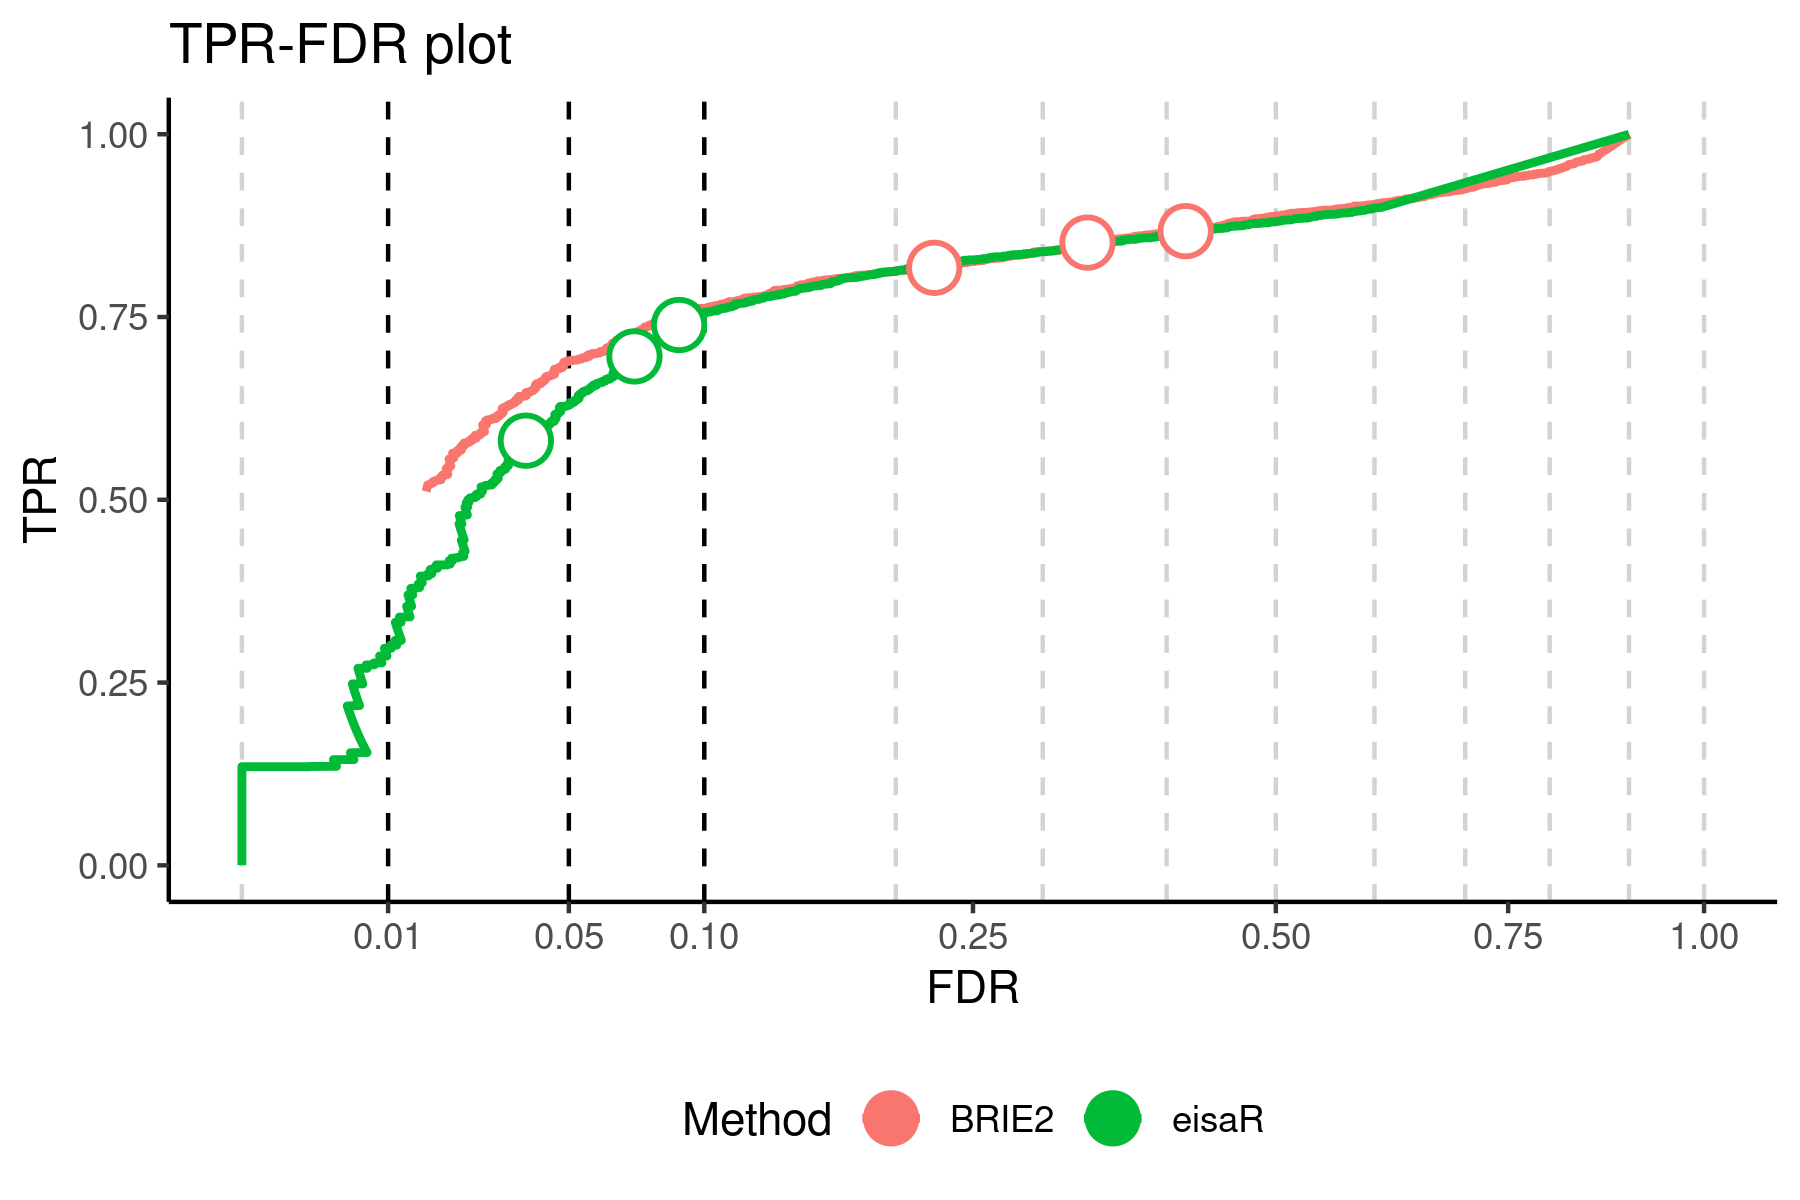
\includegraphics[width=6in,height=3.8in]{../figures/simulation/naive_simulation_DGE_FDR.png}
\end{center}
\caption{TPR v. FDR plot of \emph{BRIE2} and \emph{eisaR} in the initial simulation with DGE}
\label{fig:naive_sim_DGE_FDR}
\end{figure}
\FloatBarrier

\subsection{Simulation with mapping uncertainty} \label{soph_sim}
As a next step, multi-mapping uncertainty was introduced in to the two simulated data sets. First, \emph{minnow} was used to simulate new reads from the previously simulated data sets. Second, we used \emph{alevin-fry} to align the generated read files to the reference genome and for quantification of the reads. The newly generated data sets were then run on the aforementioned methods to identify differential genes. 

Figure \ref{fig:soph_sim_ROC} shows the performance of all four methods without DGE. For visualization purposes we decided to omit results where spliced and unspliced counts are very similar because it is very hard to detect a differential effect. Therefore, only results are plotted where there is a minimum difference of 0.2 between spliced and unspliced counts. From the ROC curve we observe that \emph{DEXSeq} and \emph{DifferentialRegulation} have a similar TPR, although \emph{DEXSeq} perform slightly better. Both \emph{BRIE2} and \emph{eisaR} have a lower TPR than the other two methods. From Figure \ref{fig:soph_sim_FDR} we observe that again \emph{DEXSeq} and \emph{DifferentialRegulation} have a similar performance profile. However, \emph{DifferentialRegulation} controls better for FDR than \emph{DEXSeq}. Contrarily to before, \emph{eisaR} controls quite well for FDR, however has half the TPR compared \emph{DEXSeq} and \emph{DifferentialRegulation}. On the other hand, \emph{BRIE2} does not control well for FDR as there is strong inflation.

In the next step, we investigated how the performance changes after introduction of DGE into the data set. Figure \ref{fig:soph_sim_DGE_ROC} shows the ROC curve for all four methods. From the Figure we observe that the difference in TPR between \emph{DEXSeq} and \emph{DifferentialRegulation} is smaller than before. On the other hand, the performance based on TPR is approximately the same as before for \emph{BRIE2} and \emph{eisaR}. From Figure \ref{fig:soph_sim_DGE_FDR} it is shown that \emph{DifferentialRegulation} still controls well for FDR, whereas the other three methods do not. The introduction of DGE as a nuisance parameter seems to affect the performance of \emph{DEXSeq} and \emph{eisaR} quite substantially in terms of FDR calibration as FDR is almost doubled to before. The FDR calibration for \emph{BRIE2} was not affected by DGE, although it was not well calibrated to begin with.

\begin{figure}[!htb]
\begin{center}
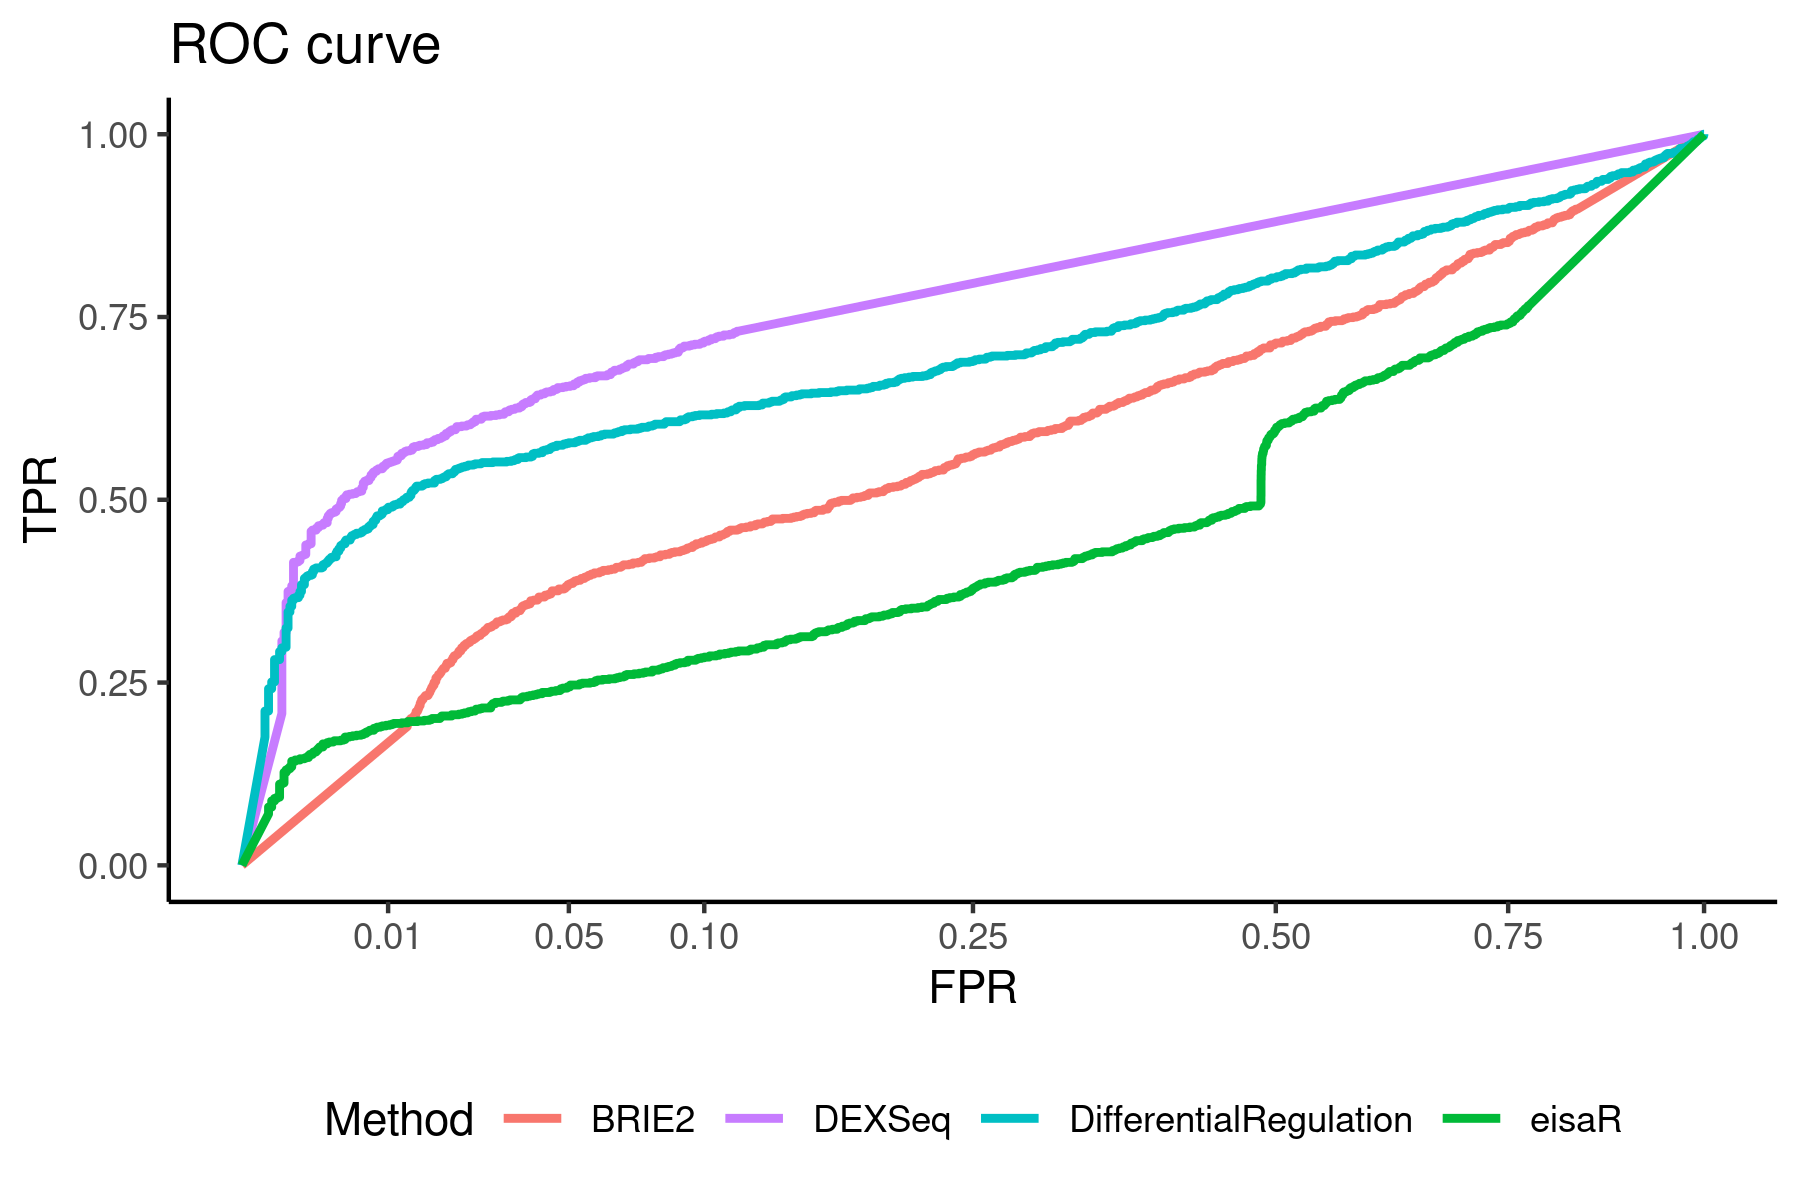
\includegraphics[width=6in,height=4in]{../figures/simulation/minnow_simulation_ROC.png}
\end{center}
\caption{ROC curve of \emph{BRIE2}, \emph{DEXSeq}, \emph{DifferentialRegulation} and \emph{eisaR} in the sophisticated simulation without DGE}
\label{fig:soph_sim_ROC}
\end{figure}

\begin{figure}[!htb]
\begin{center}
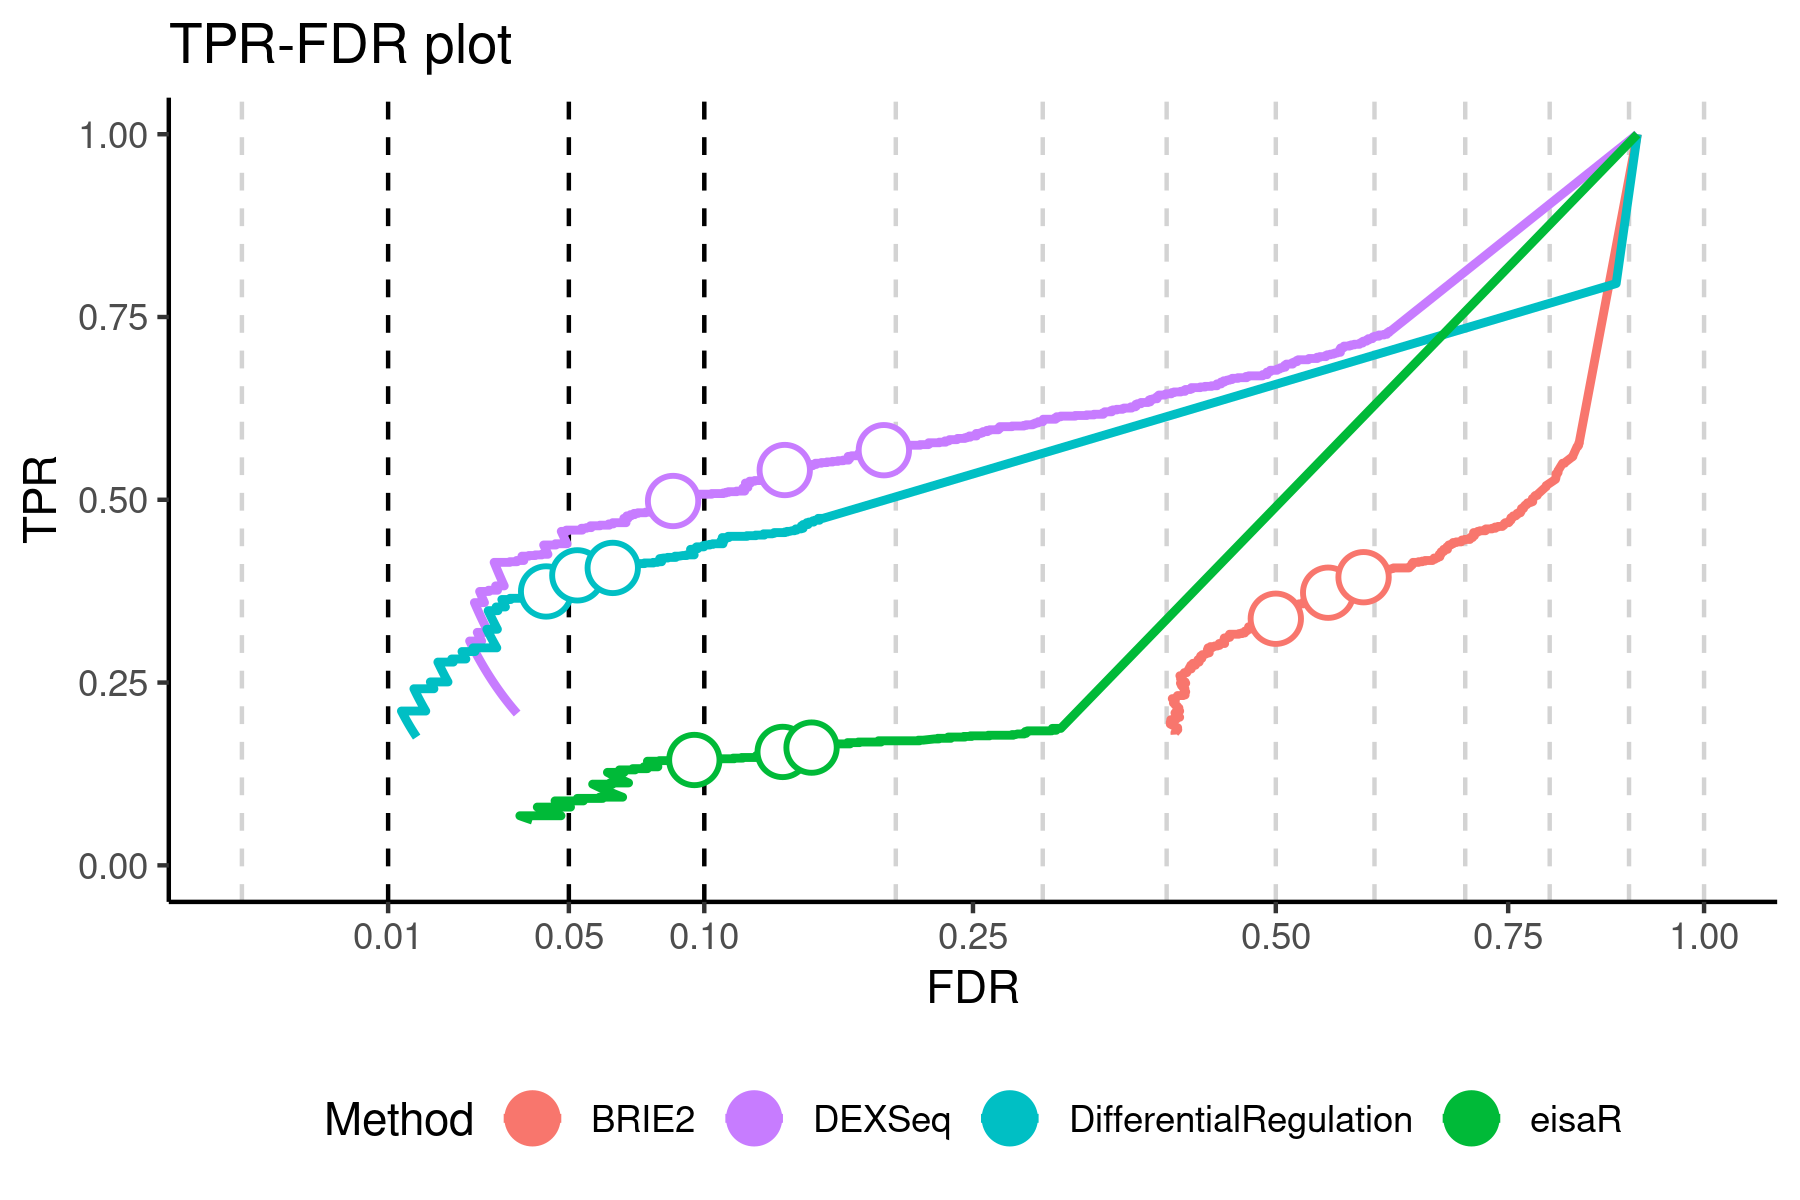
\includegraphics[width=6in,height=4in]{../figures/simulation/minnow_simulation_FDR.png}
\end{center}
\caption{TPR v. FDR plot of \emph{BRIE2}, \emph{DEXSeq}, \emph{DifferentialRegulation} and \emph{eisaR} in the sophisticated simulation without DGE}
\label{fig:soph_sim_FDR}
\end{figure}

\begin{figure}[!htb]
\begin{center}
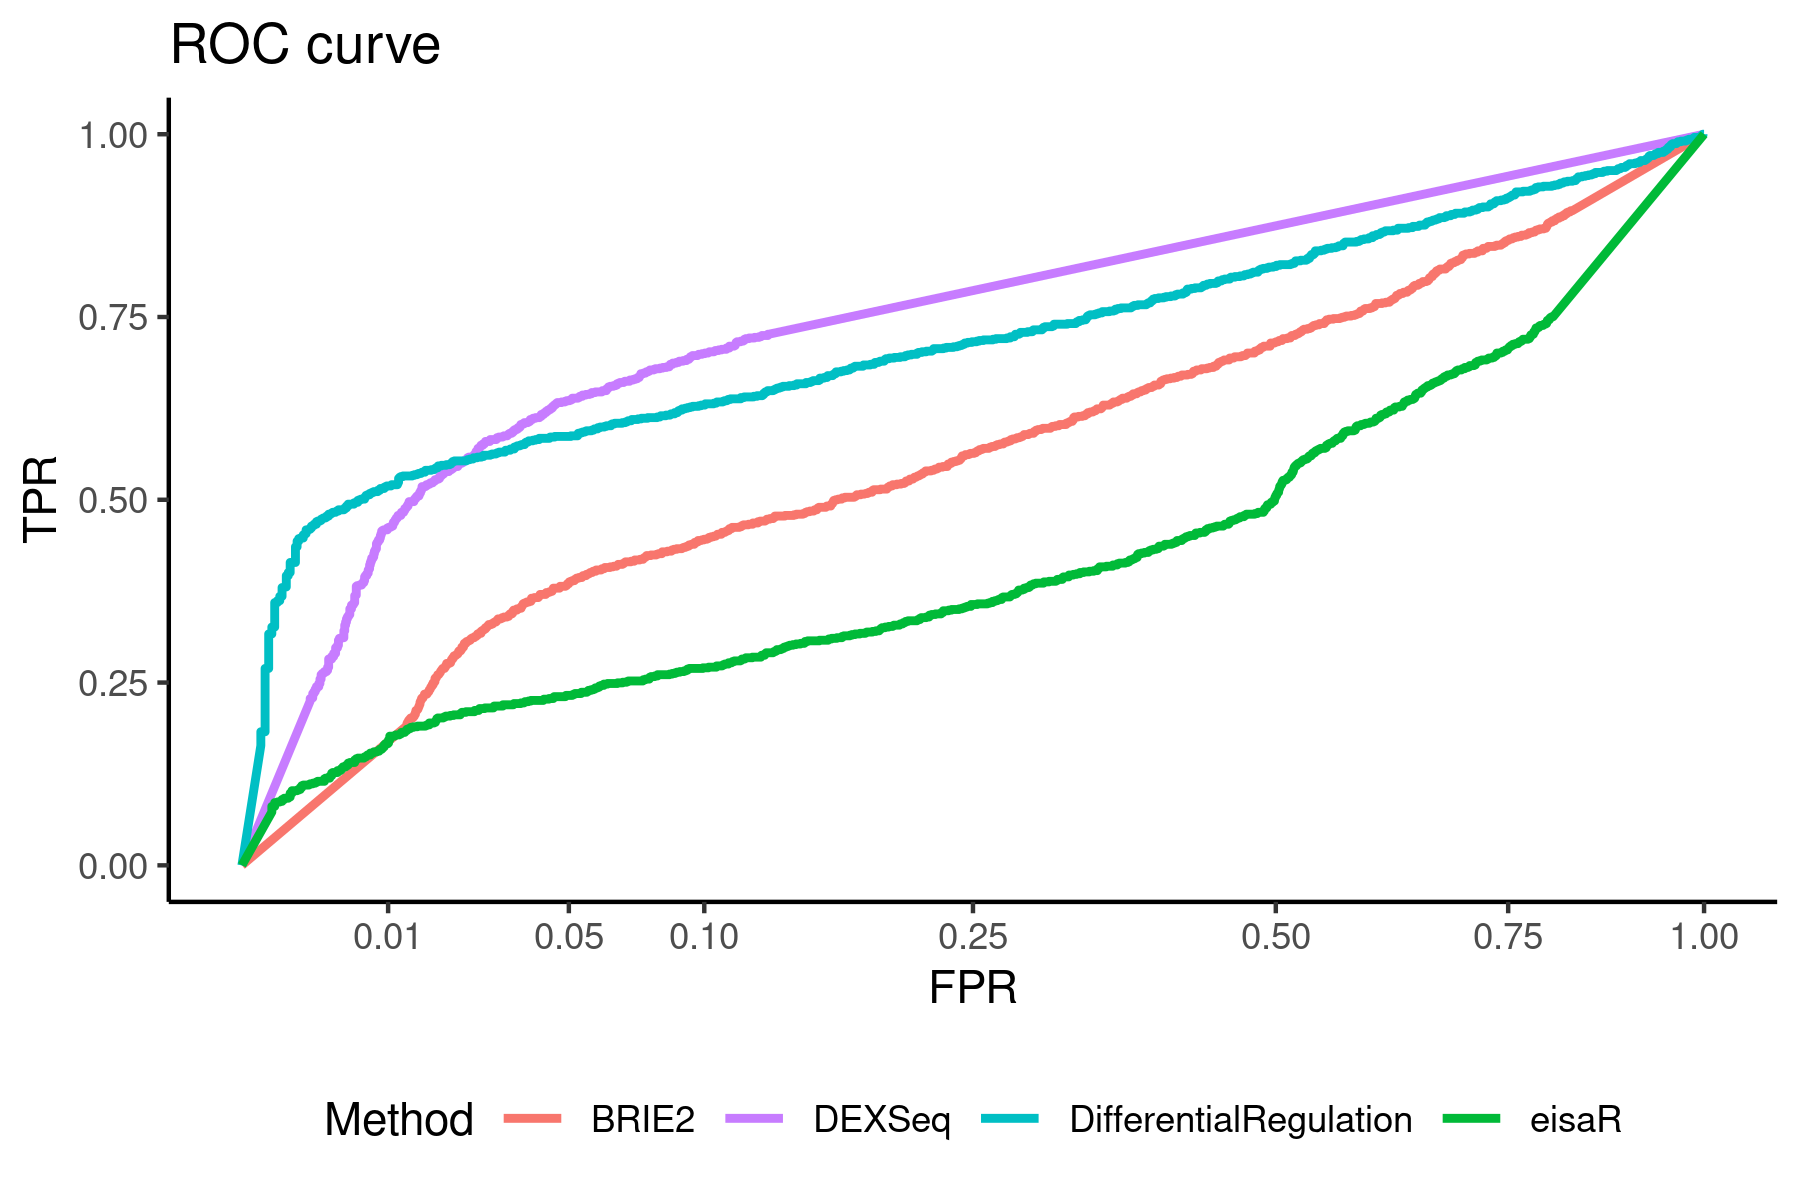
\includegraphics[width=6in,height=4in]{../figures/simulation/minnow_simulation_DGE_ROC.png}
\end{center}
\caption{ROC curve of \emph{BRIE2}, \emph{DEXSeq}, \emph{DifferentialRegulation} and \emph{eisaR} in the sophisticated simulation with DGE}
\label{fig:soph_sim_DGE_ROC}
\end{figure}

\begin{figure}[!htb]
\begin{center}
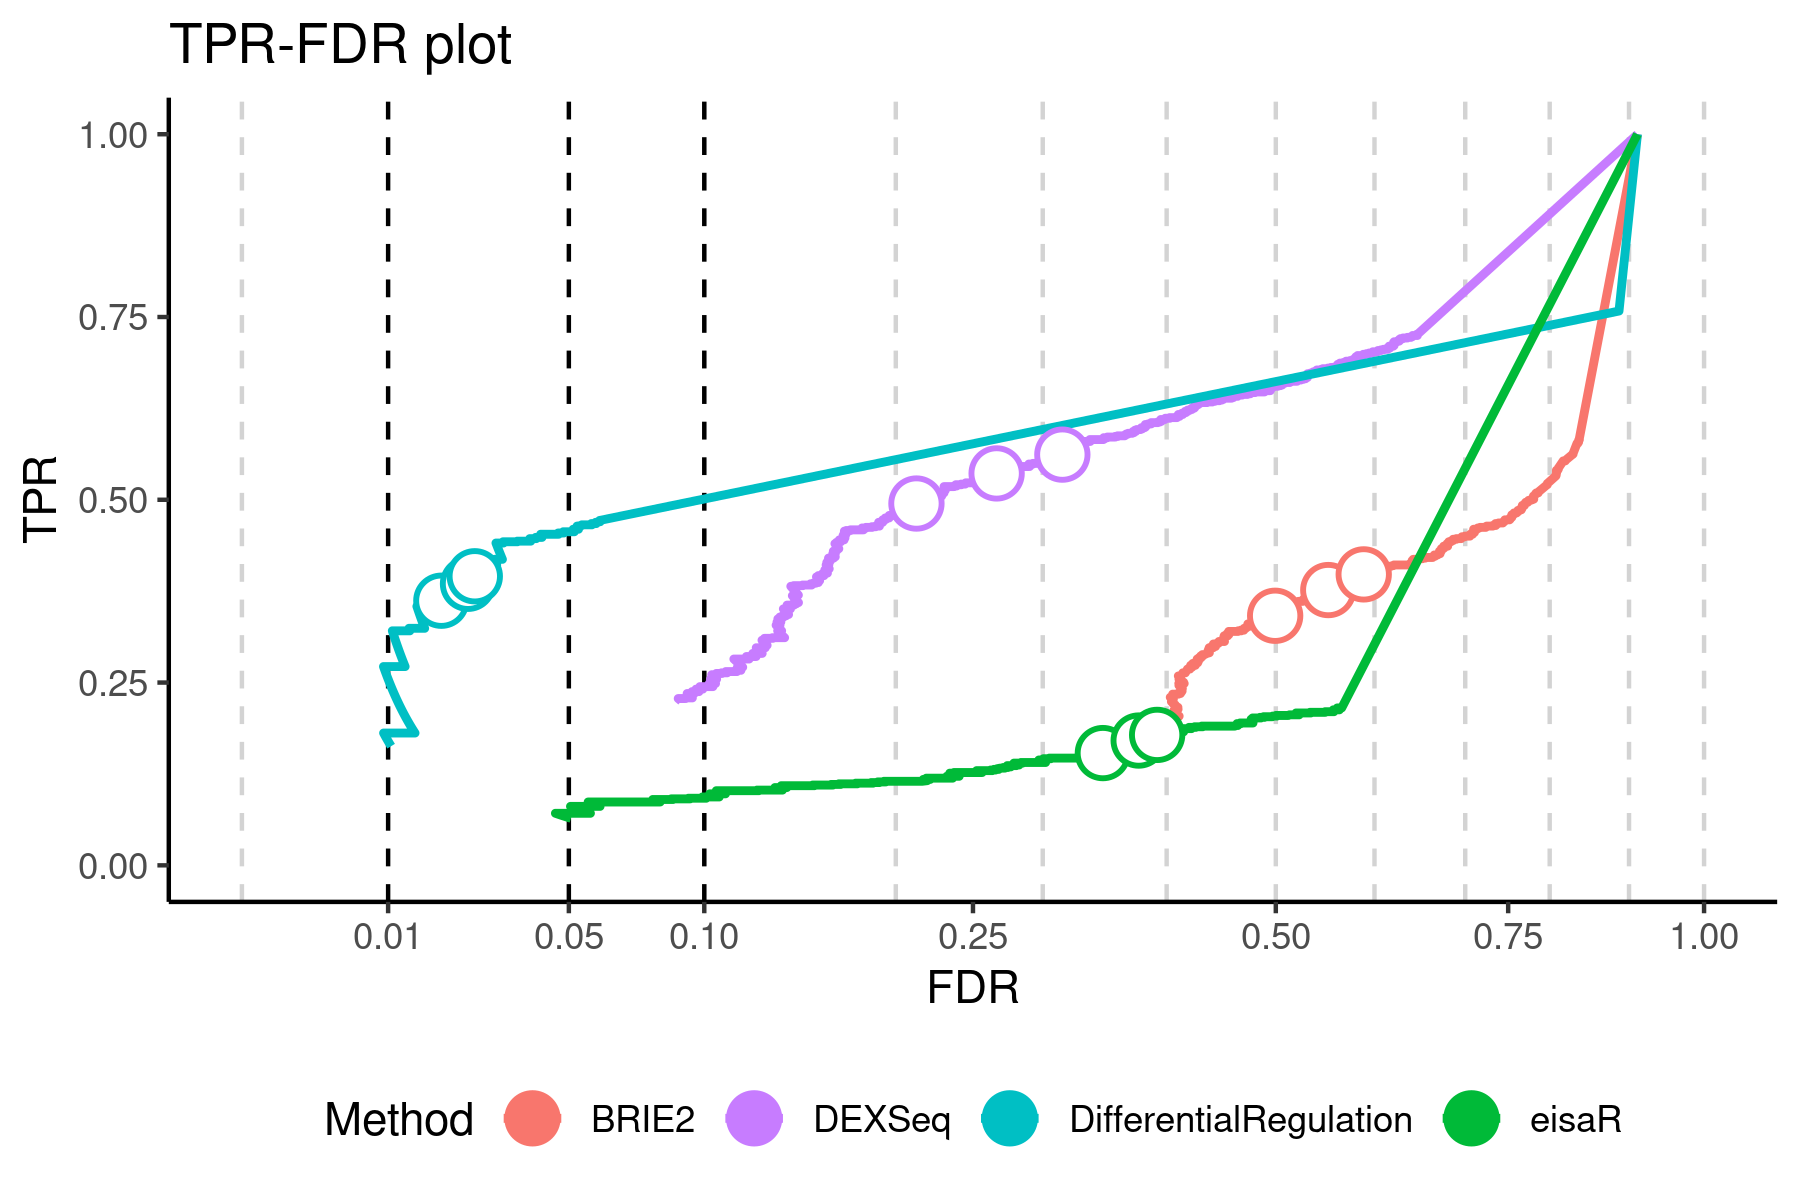
\includegraphics[width=6in,height=3.8in]{../figures/simulation/minnow_simulation_DGE_FDR.png}
\end{center}
\caption{TPR v. FDR plot of \emph{BRIE2}, \emph{DEXSeq}, \emph{eisaR} and \emph{DifferentialRegulation} in the sophisticated simulation with DGE}
\label{fig:soph_sim_DGE_FDR}
\end{figure}

Furthermore, in order to assess how overall gene abundance affects results, we stratified the previous results by gene expression and evaluated performance, separately, for lowly, medium and highly abundant genes. This is achieved by separating results according to overall gene abundance into 3 groups, based on the quantiles of levels 1/3 and 2/3; in particular, lowly abundant genes have abundance below the first quantile (of level 1/3), moderately expressed genes have expression between the two quantiles, while highly abundant genes have expression above the second quantile (of level 2/3).

Figures \ref{fig:soph_sim_FDR_low} to \ref{fig:soph_sim_DGE_FDR_high} show the results stratified by the level of gene abundance. The Figures show that performance is consistent across gene abundance levels for \emph{DifferentialRegulation}. TPR increases only marginally, which is expected as more data usually implies higher statistical power and FDR is also stable across gene abundance levels. Overall, \emph{DifferentialRegulation} is not substantially impacted by gene abundance. For \emph{DEXSeq}, TPR and FDR are both increasing as gene abundance rises. This effect is even larger for the simulation with DGE. For \emph{BRIE2} there is a significant increase of TPR from low to highly abundant genes, however, the FDR is badly calibrated. With \emph{eisaR} there is a marginal increase of TPR, whereas FDR is only slightly inflated without DGE. On the other hand, FDR is strongly inflated with DGE as gene abundance rises, which is expected as \emph{eisaR} tests on absolute abundance of spliced and unspliced counts, therefore it detects both differentially regulated and differentially expressed genes.

In this part we investigated how robust the methods are to gene abundance with and without DGE. We concluded that the performance of \emph{BRIE2} is low in all cases. \emph{eisaR} has a low TPR but FDR is generally well calibrated without DGE. \emph{DEXSeq} has good TPR and mild inflation of FDR without DGE, however, there is a strong increase in FDR with DGE. Generally, both TPR and FDR are increasing as gene abundance level rises. On the other hand, \emph{DifferentialRegulation} is the only method with good TPR and well calibrated FDR with and without DGE across all levels of gene abundance.

\begin{figure}[!htb]
\begin{center}
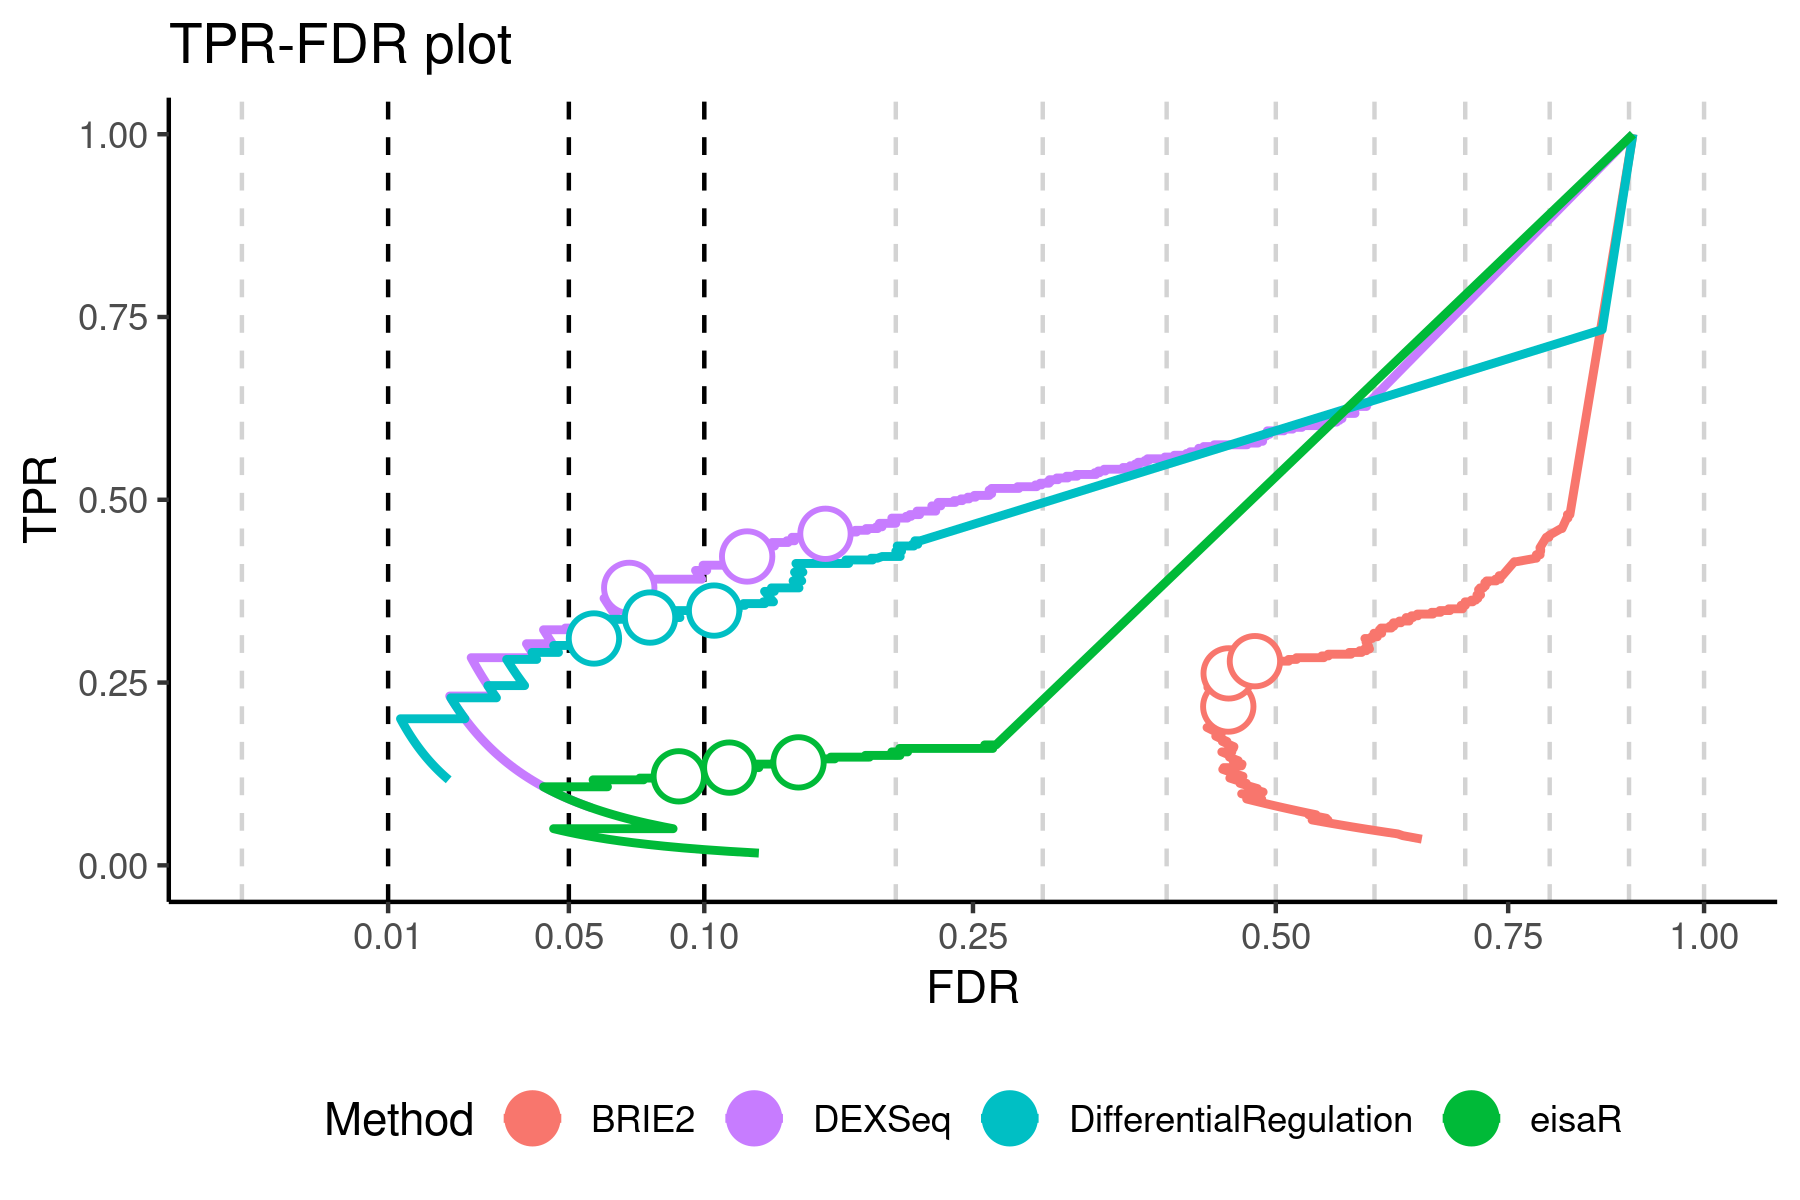
\includegraphics[width=6in,height=3.8in]{../figures/simulation/minnow_simulation_low_FDR.png}
\end{center}
\caption{TPR v. FDR plot of \emph{BRIE2}, \emph{DEXSeq}, \emph{DifferentialRegulation} and \emph{eisaR} in the sophisticated simulation for the lowly expressed genes in the stratified analysis}
\label{fig:soph_sim_FDR_low}
\end{figure}

\begin{figure}[!htb]
\begin{center}
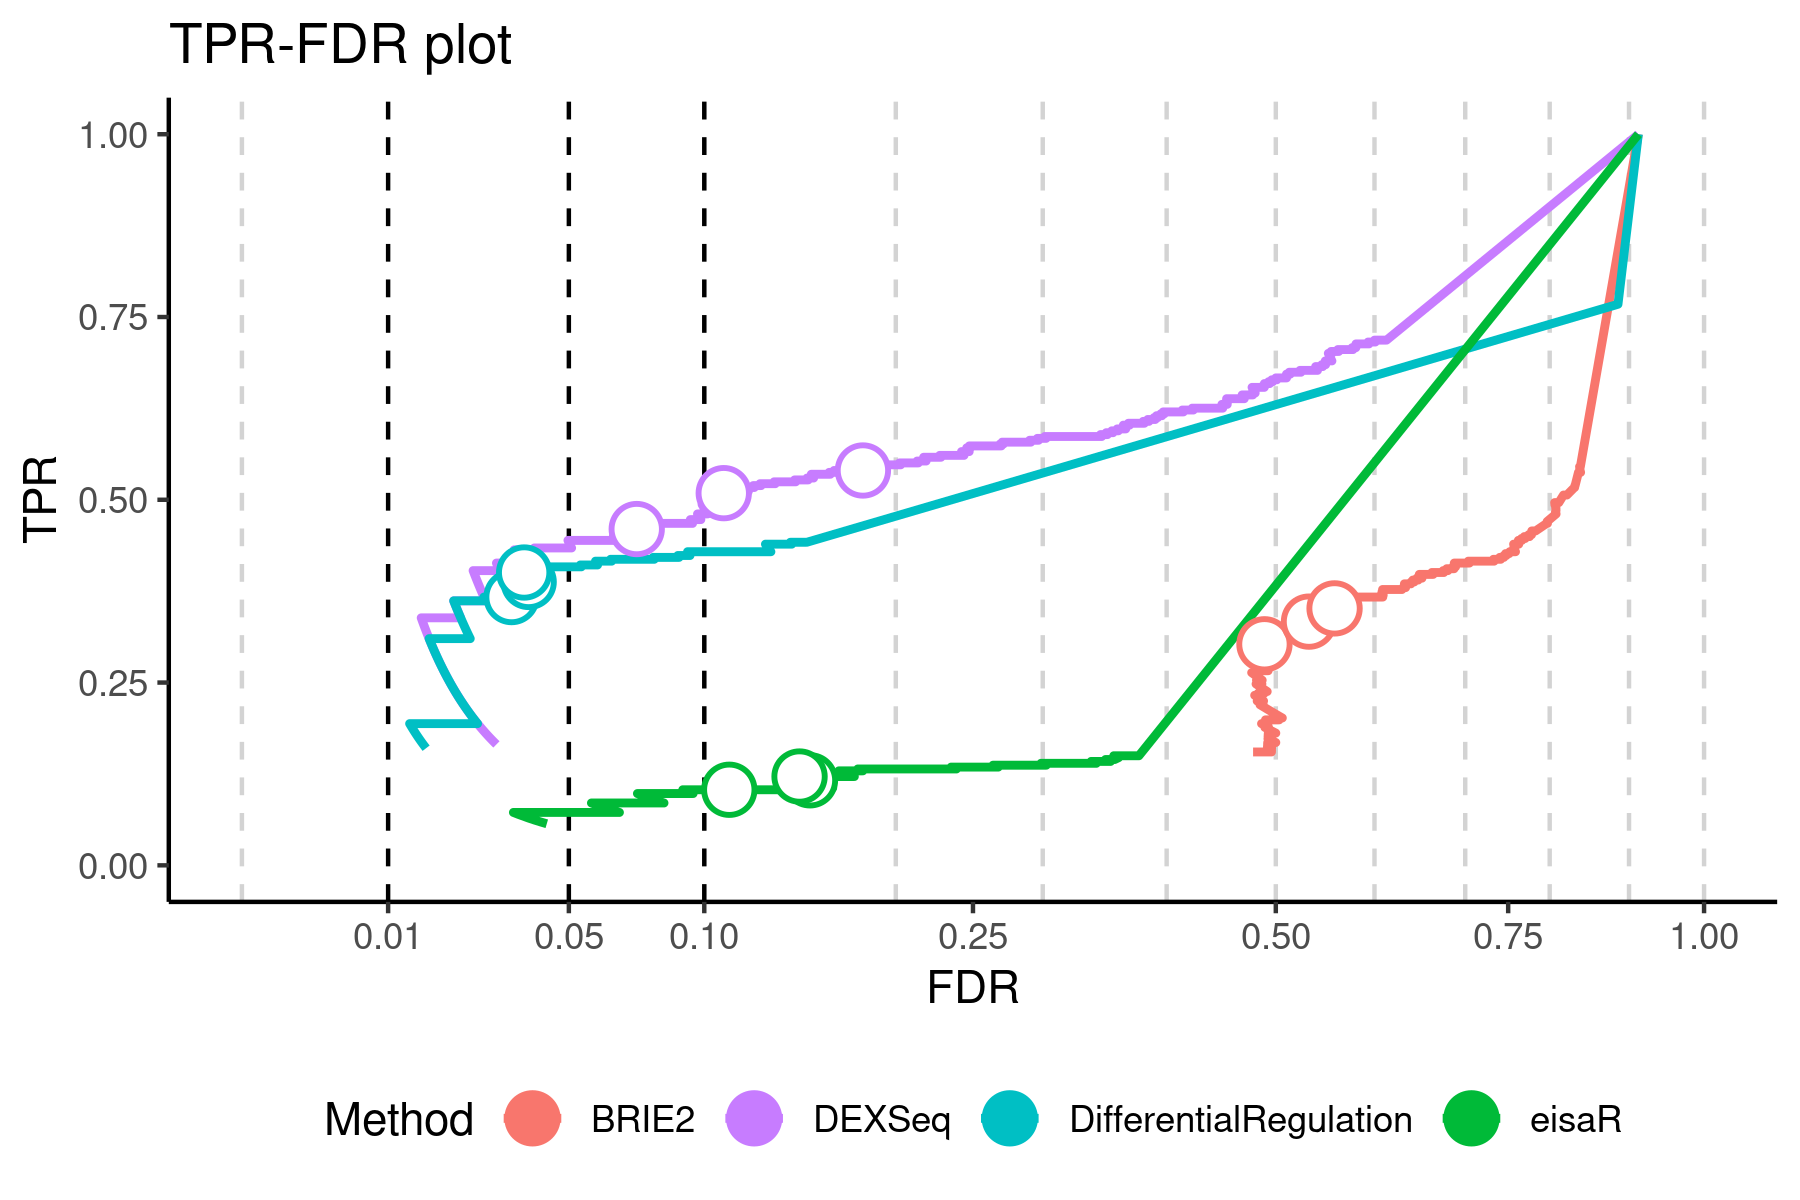
\includegraphics[width=6in,height=3.8in]{../figures/simulation/minnow_simulation_mod_FDR.png}
\end{center}
\caption{TPR v. FDR plot of \emph{BRIE2}, \emph{DEXSeq}, \emph{DifferentialRegulation} and \emph{eisaR} in the sophisticated simulation for the moderately expressed genes in the stratified analysis}
\label{fig:soph_sim_FDR_mod}
\end{figure}

\begin{figure}[!htb]
\begin{center}
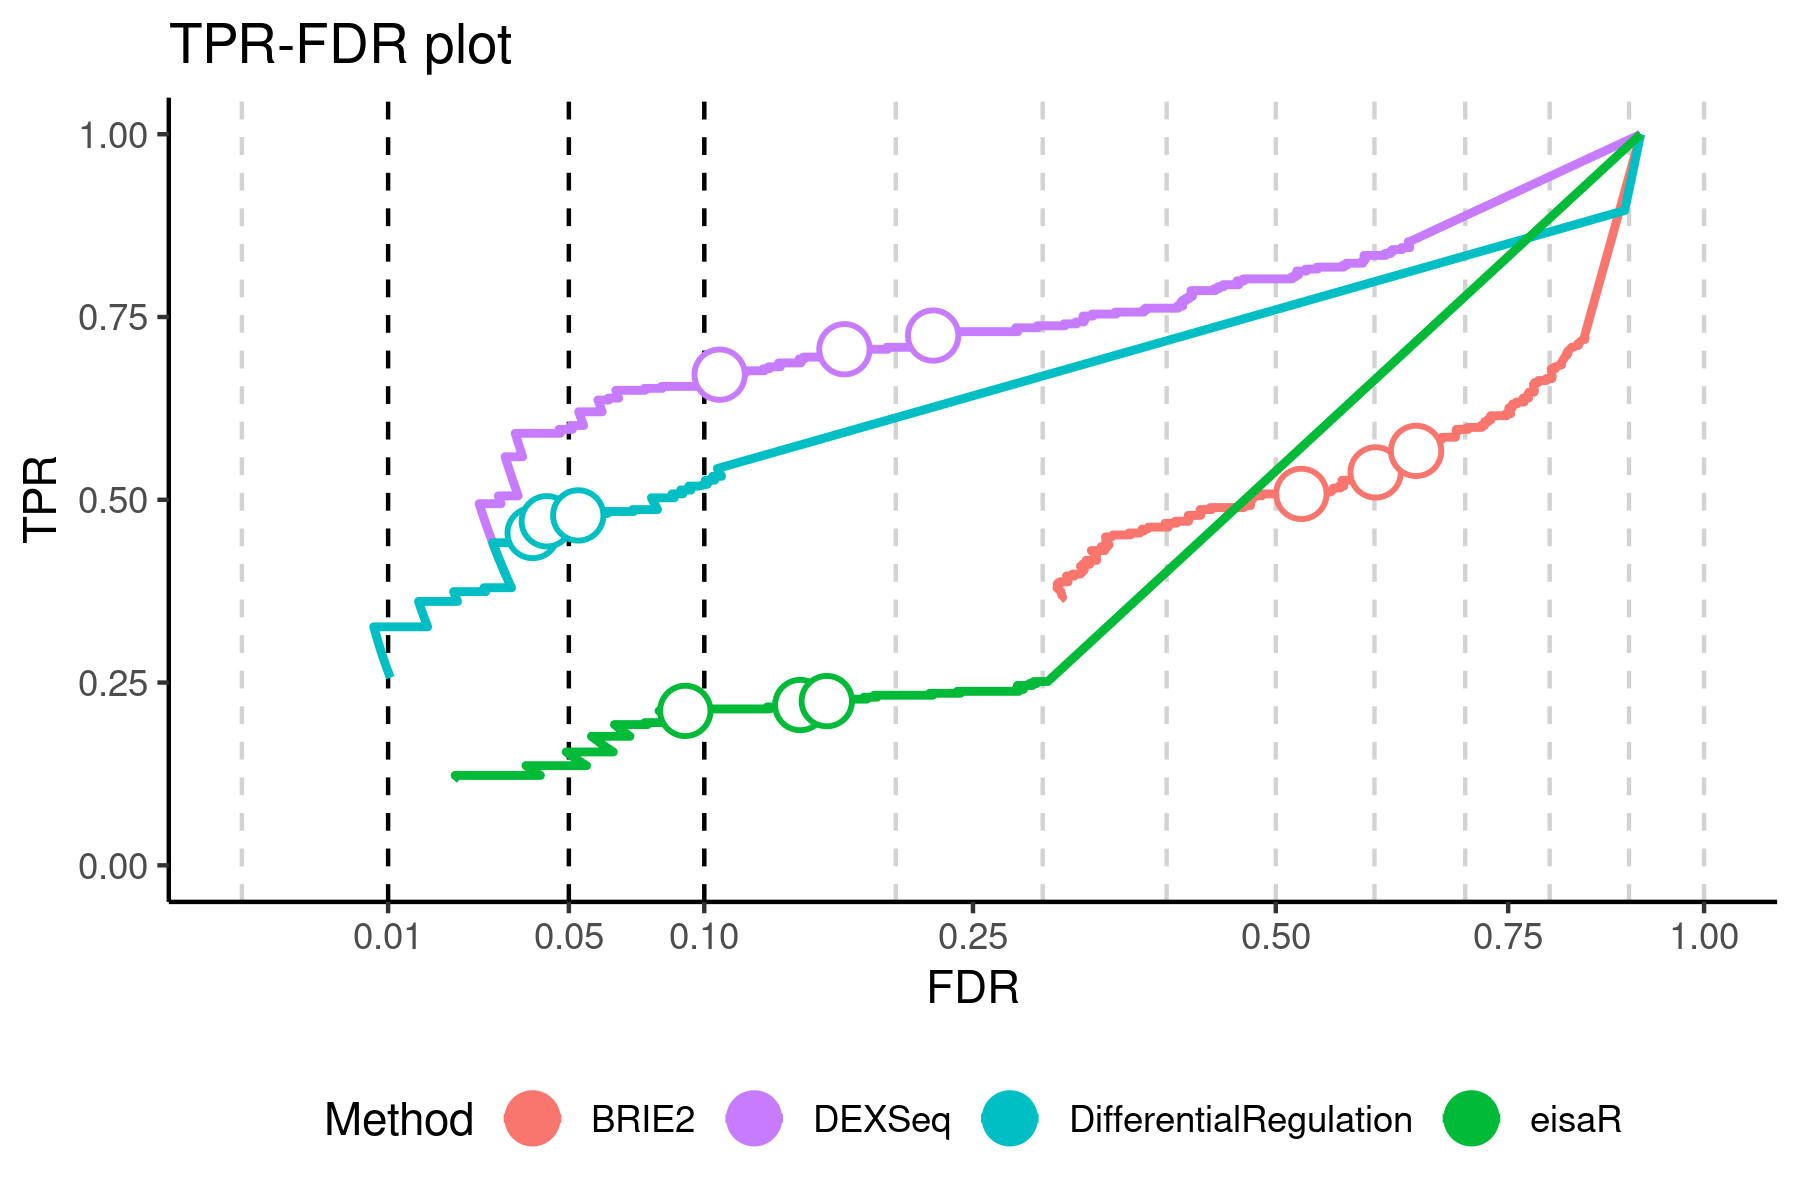
\includegraphics[width=6in,height=3.8in]{../figures/simulation/minnow_simulation_high_FDR.png}
\end{center}
\caption{TPR v. FDR plot of \emph{BRIE2}, \emph{DEXSeq}, \emph{DifferentialRegulation} and \emph{eisaR} in the sophisticated simulation for the highly expressed genes in the stratified analysis}
\label{fig:soph_sim_FDR_high}
\end{figure}

\begin{figure}[!htb]
\begin{center}
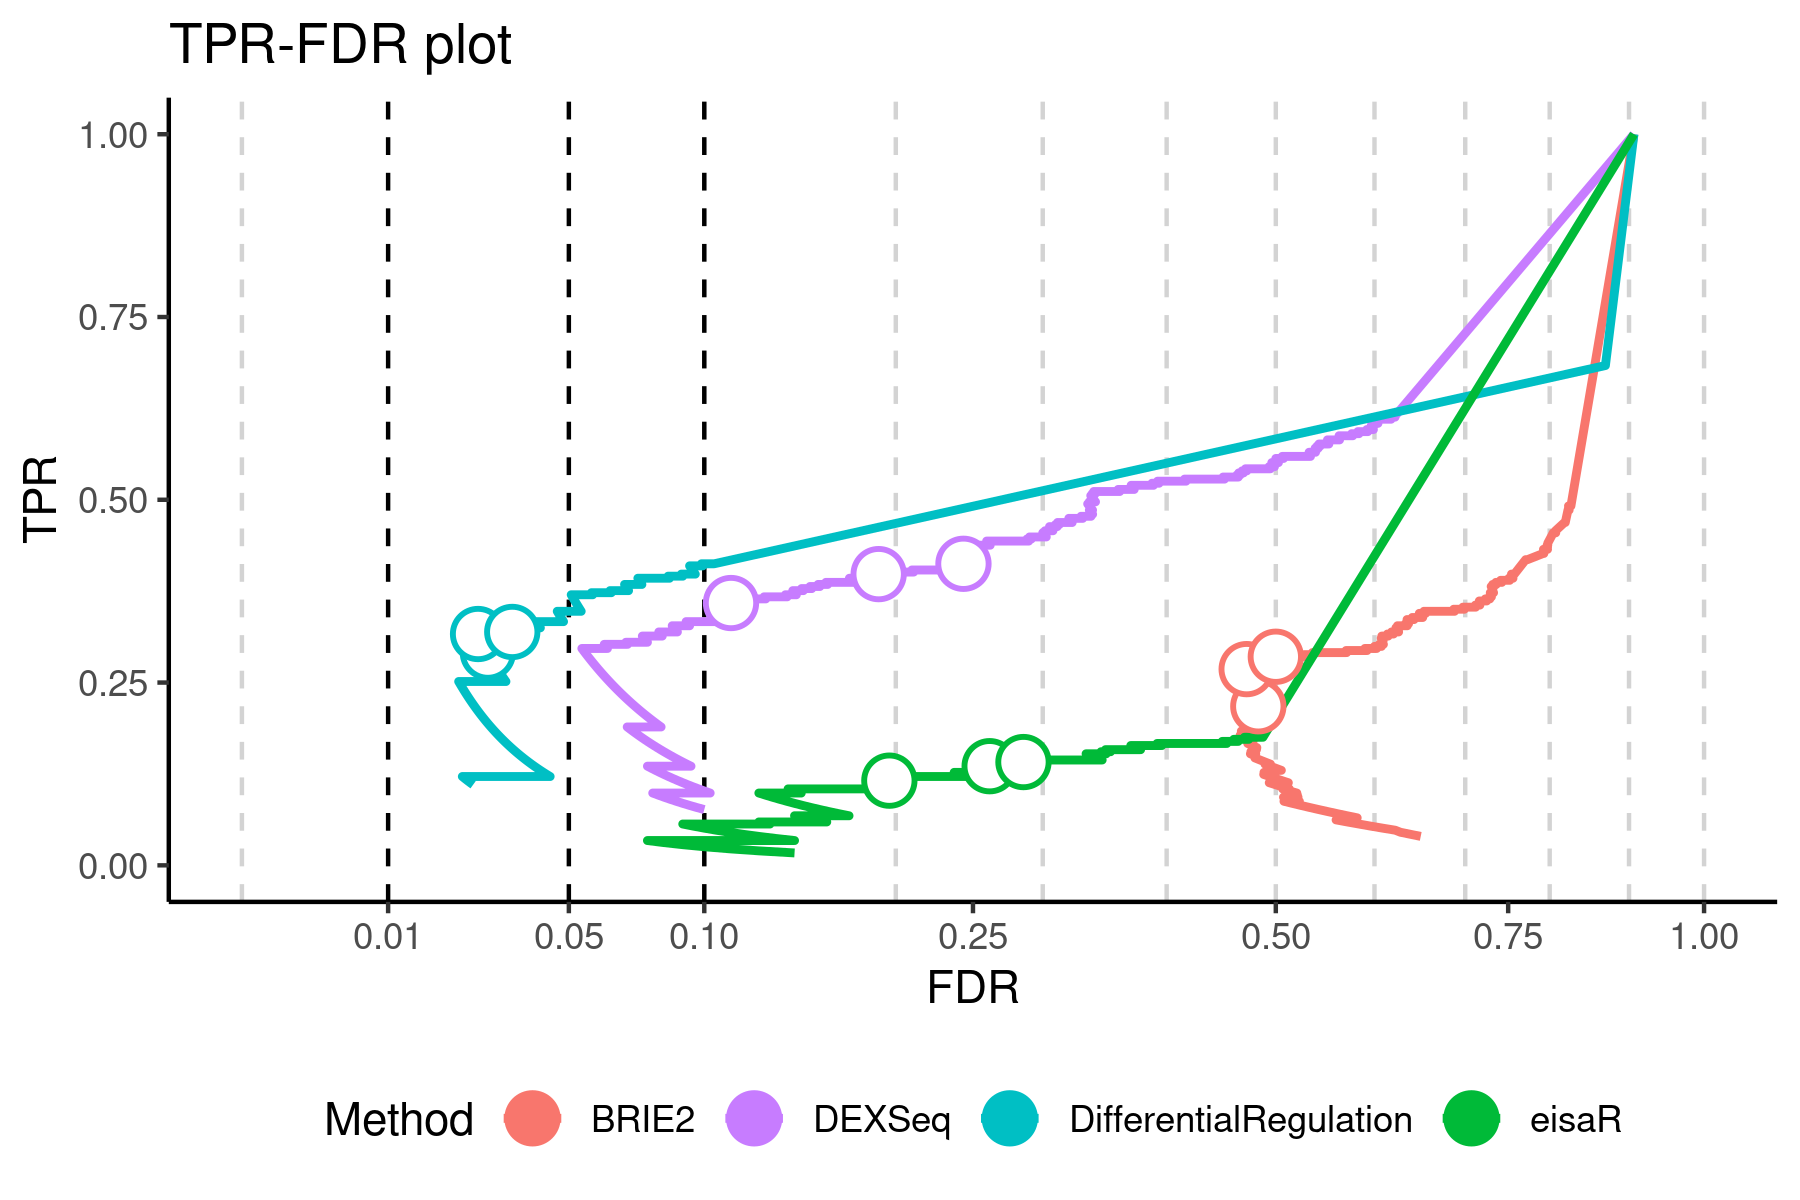
\includegraphics[width=6in,height=3.8in]{../figures/simulation/minnow_simulation_low_DGE_FDR.png}
\end{center}
\caption{TPR v. FDR plot of \emph{BRIE2}, \emph{DEXSeq}, \emph{DifferentialRegulation} and \emph{eisaR} in the sophisticated simulation for the lowly expressed genes in the stratified analysis with DGE}
\label{fig:soph_sim_DGE_FDR_low}
\end{figure}

\begin{figure}[!htb]
\begin{center}
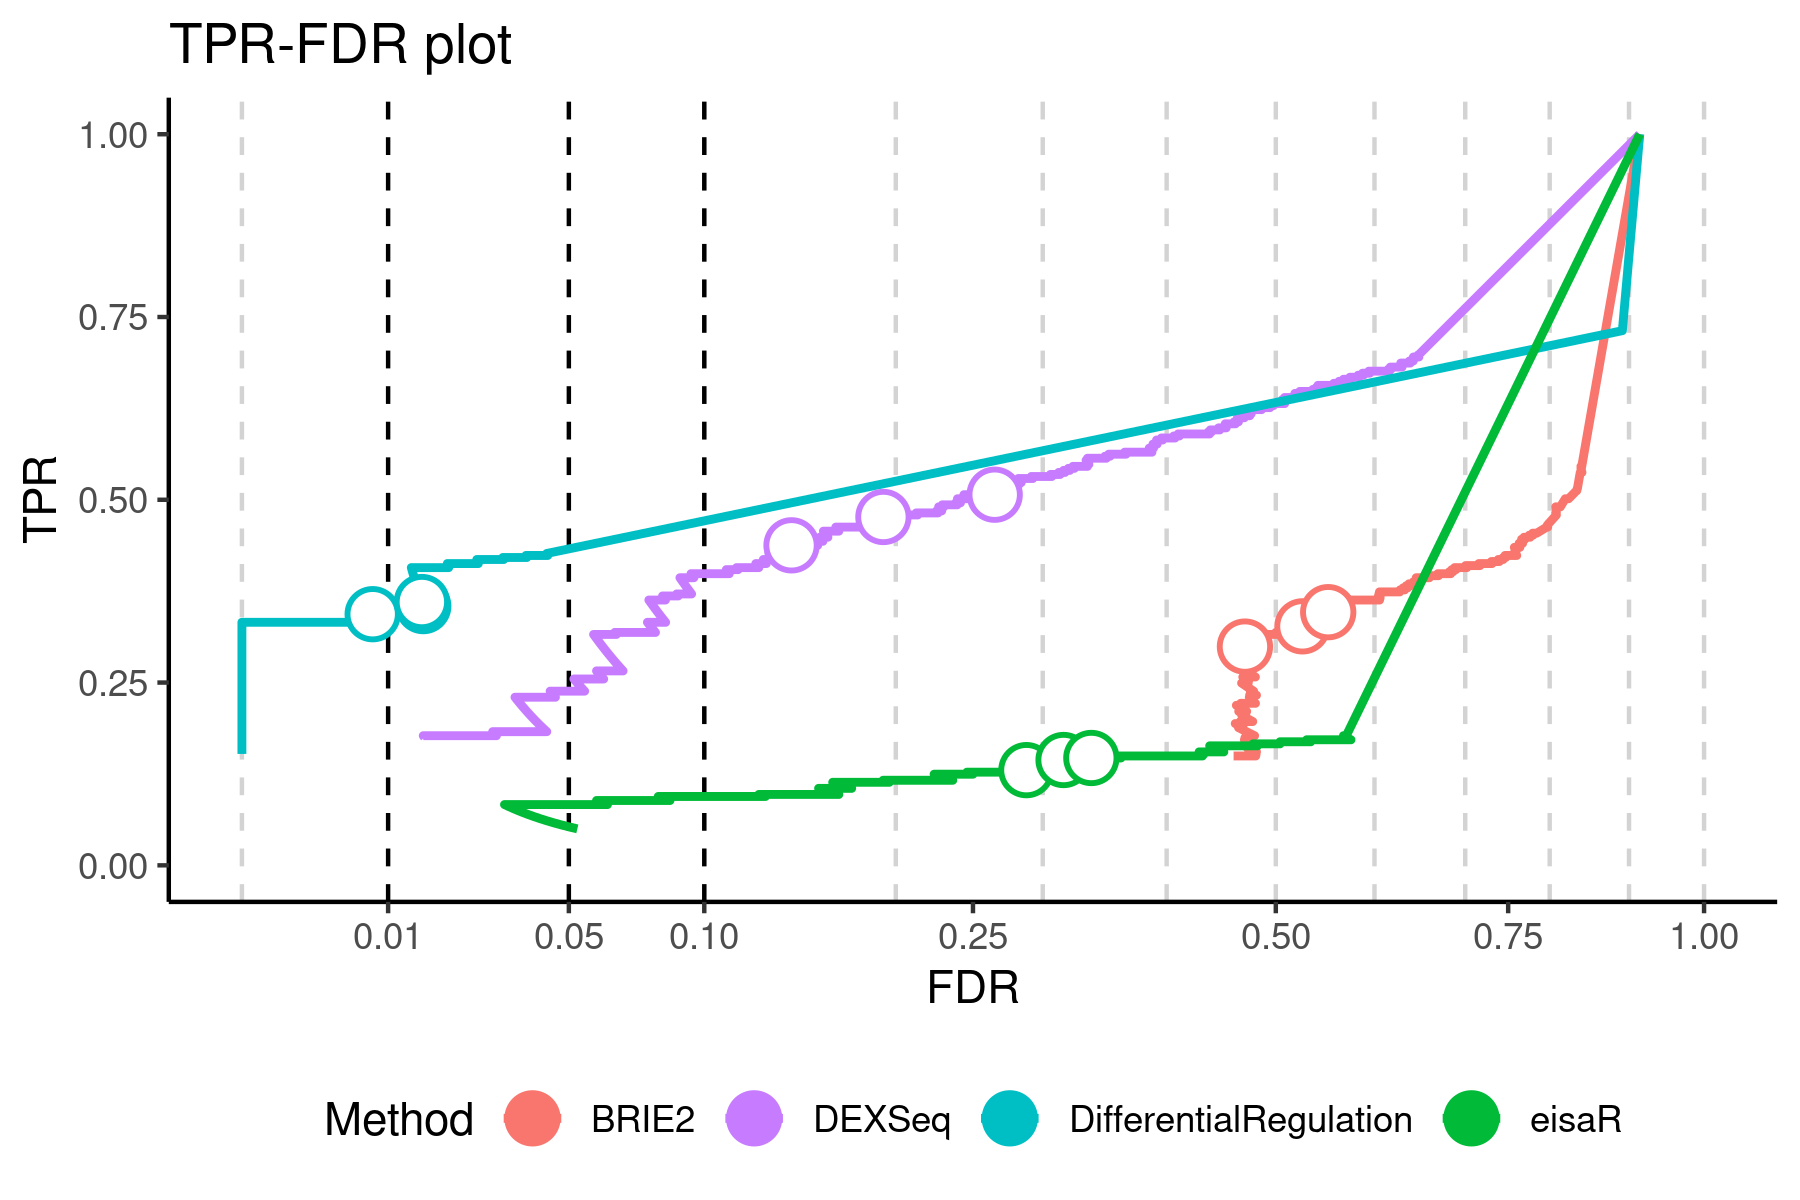
\includegraphics[width=6in,height=3.8in]{../figures/simulation/minnow_simulation_mod_DGE_FDR.png}
\end{center}
\caption{TPR v. FDR plot of \emph{BRIE2}, \emph{DEXSeq}, \emph{DifferentialRegulation} and \emph{eisaR} in the sophisticated simulation for the moderately expressed genes in the stratified analysis with DGE}
\label{fig:soph_sim_DGE_FDR_mod}
\end{figure}

\begin{figure}[!htb]
\begin{center}
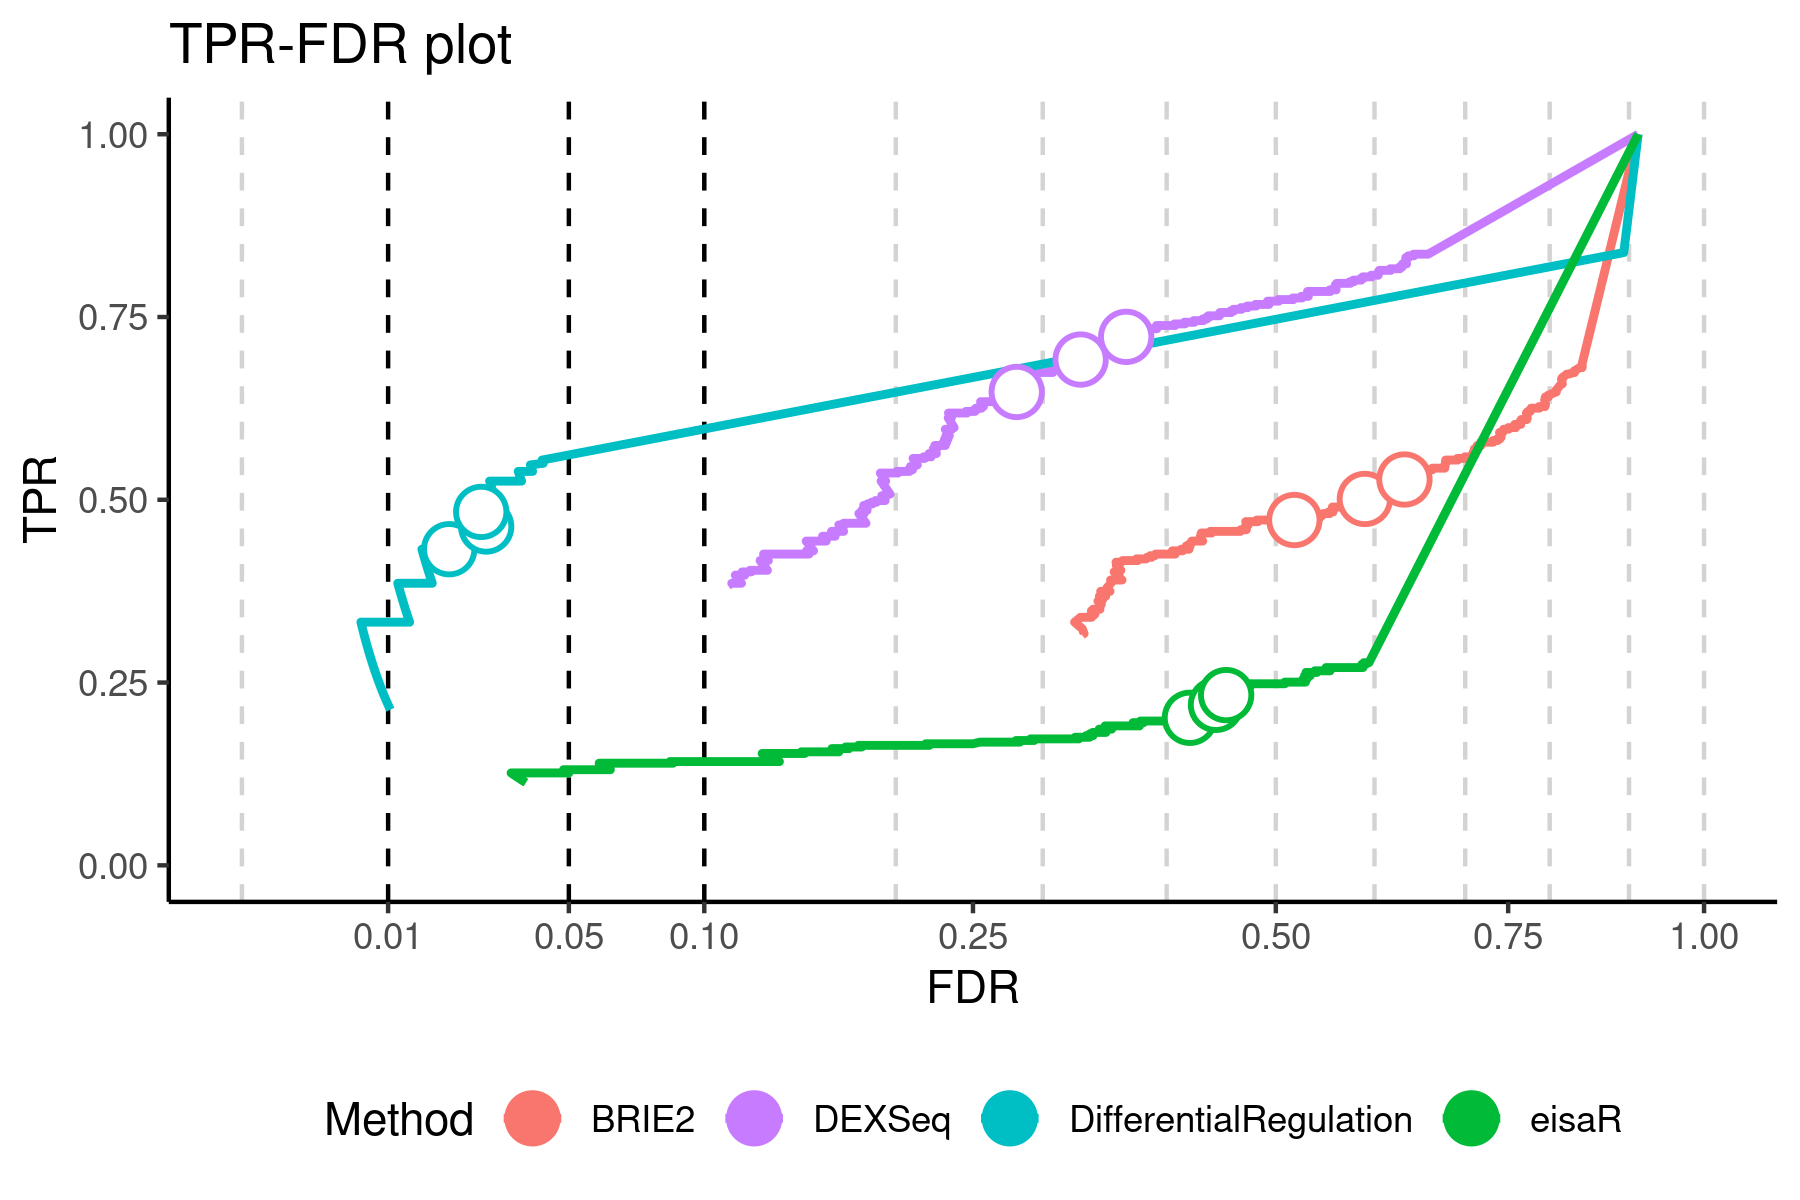
\includegraphics[width=6in,height=3.8in]{../figures/simulation/minnow_simulation_high_DGE_FDR.png}
\end{center}
\caption{TPR v. FDR plot of \emph{BRIE2}, \emph{DEXSeq}, \emph{DifferentialRegulation} and \emph{eisaR} in the sophisticated simulation for the highly expressed genes in the stratified analysis with DGE}
\label{fig:soph_sim_DGE_FDR_high}
\end{figure}
\FloatBarrier

\section{Null analysis on the mouse kidney data}
As a last step, a Null analysis was conducted on the original mouse kidney data set to evaluate the methods of on a real world data set. For that, all three possible group allocations were considered. Under the Null hypothesis $H_0$ the p-values would be uniformly distributed between zero and one, because all samples belong to the same experiment condition (i.e. normal). In particular, we were interested in checking for false positive detections which are indicated by inflated p-values towards zero. Figure \ref{fig:null_p_values} shows that the p-values are slightly inflated for the first group separation, which leads to a marginal separation between groups, as visible from the UMAP \ref{fig:UMAP_mouse_sample_id}. Further, from Figure \ref{fig:null_p_values} it is shown that for \emph{DifferentialRegulation} FPs are never inflated. However, p-values are inflated towards one, hence \emph{DifferentialRegulation} is more conservative as compared to the other methods. \emph{eisaR} is only inflated for the first group separation, but overall approximately uniformly distributed. On the other hand, \emph{BRIE2} demonstrates inflated FPs for all three group separations, which is also consistent with the results from the simulation study. \emph{DEXSeq} was not evaluated for p-value distribution as it does not provide raw p-values at gene-level, whereas the other methods do.

\begin{figure}[!htb]
\begin{center}
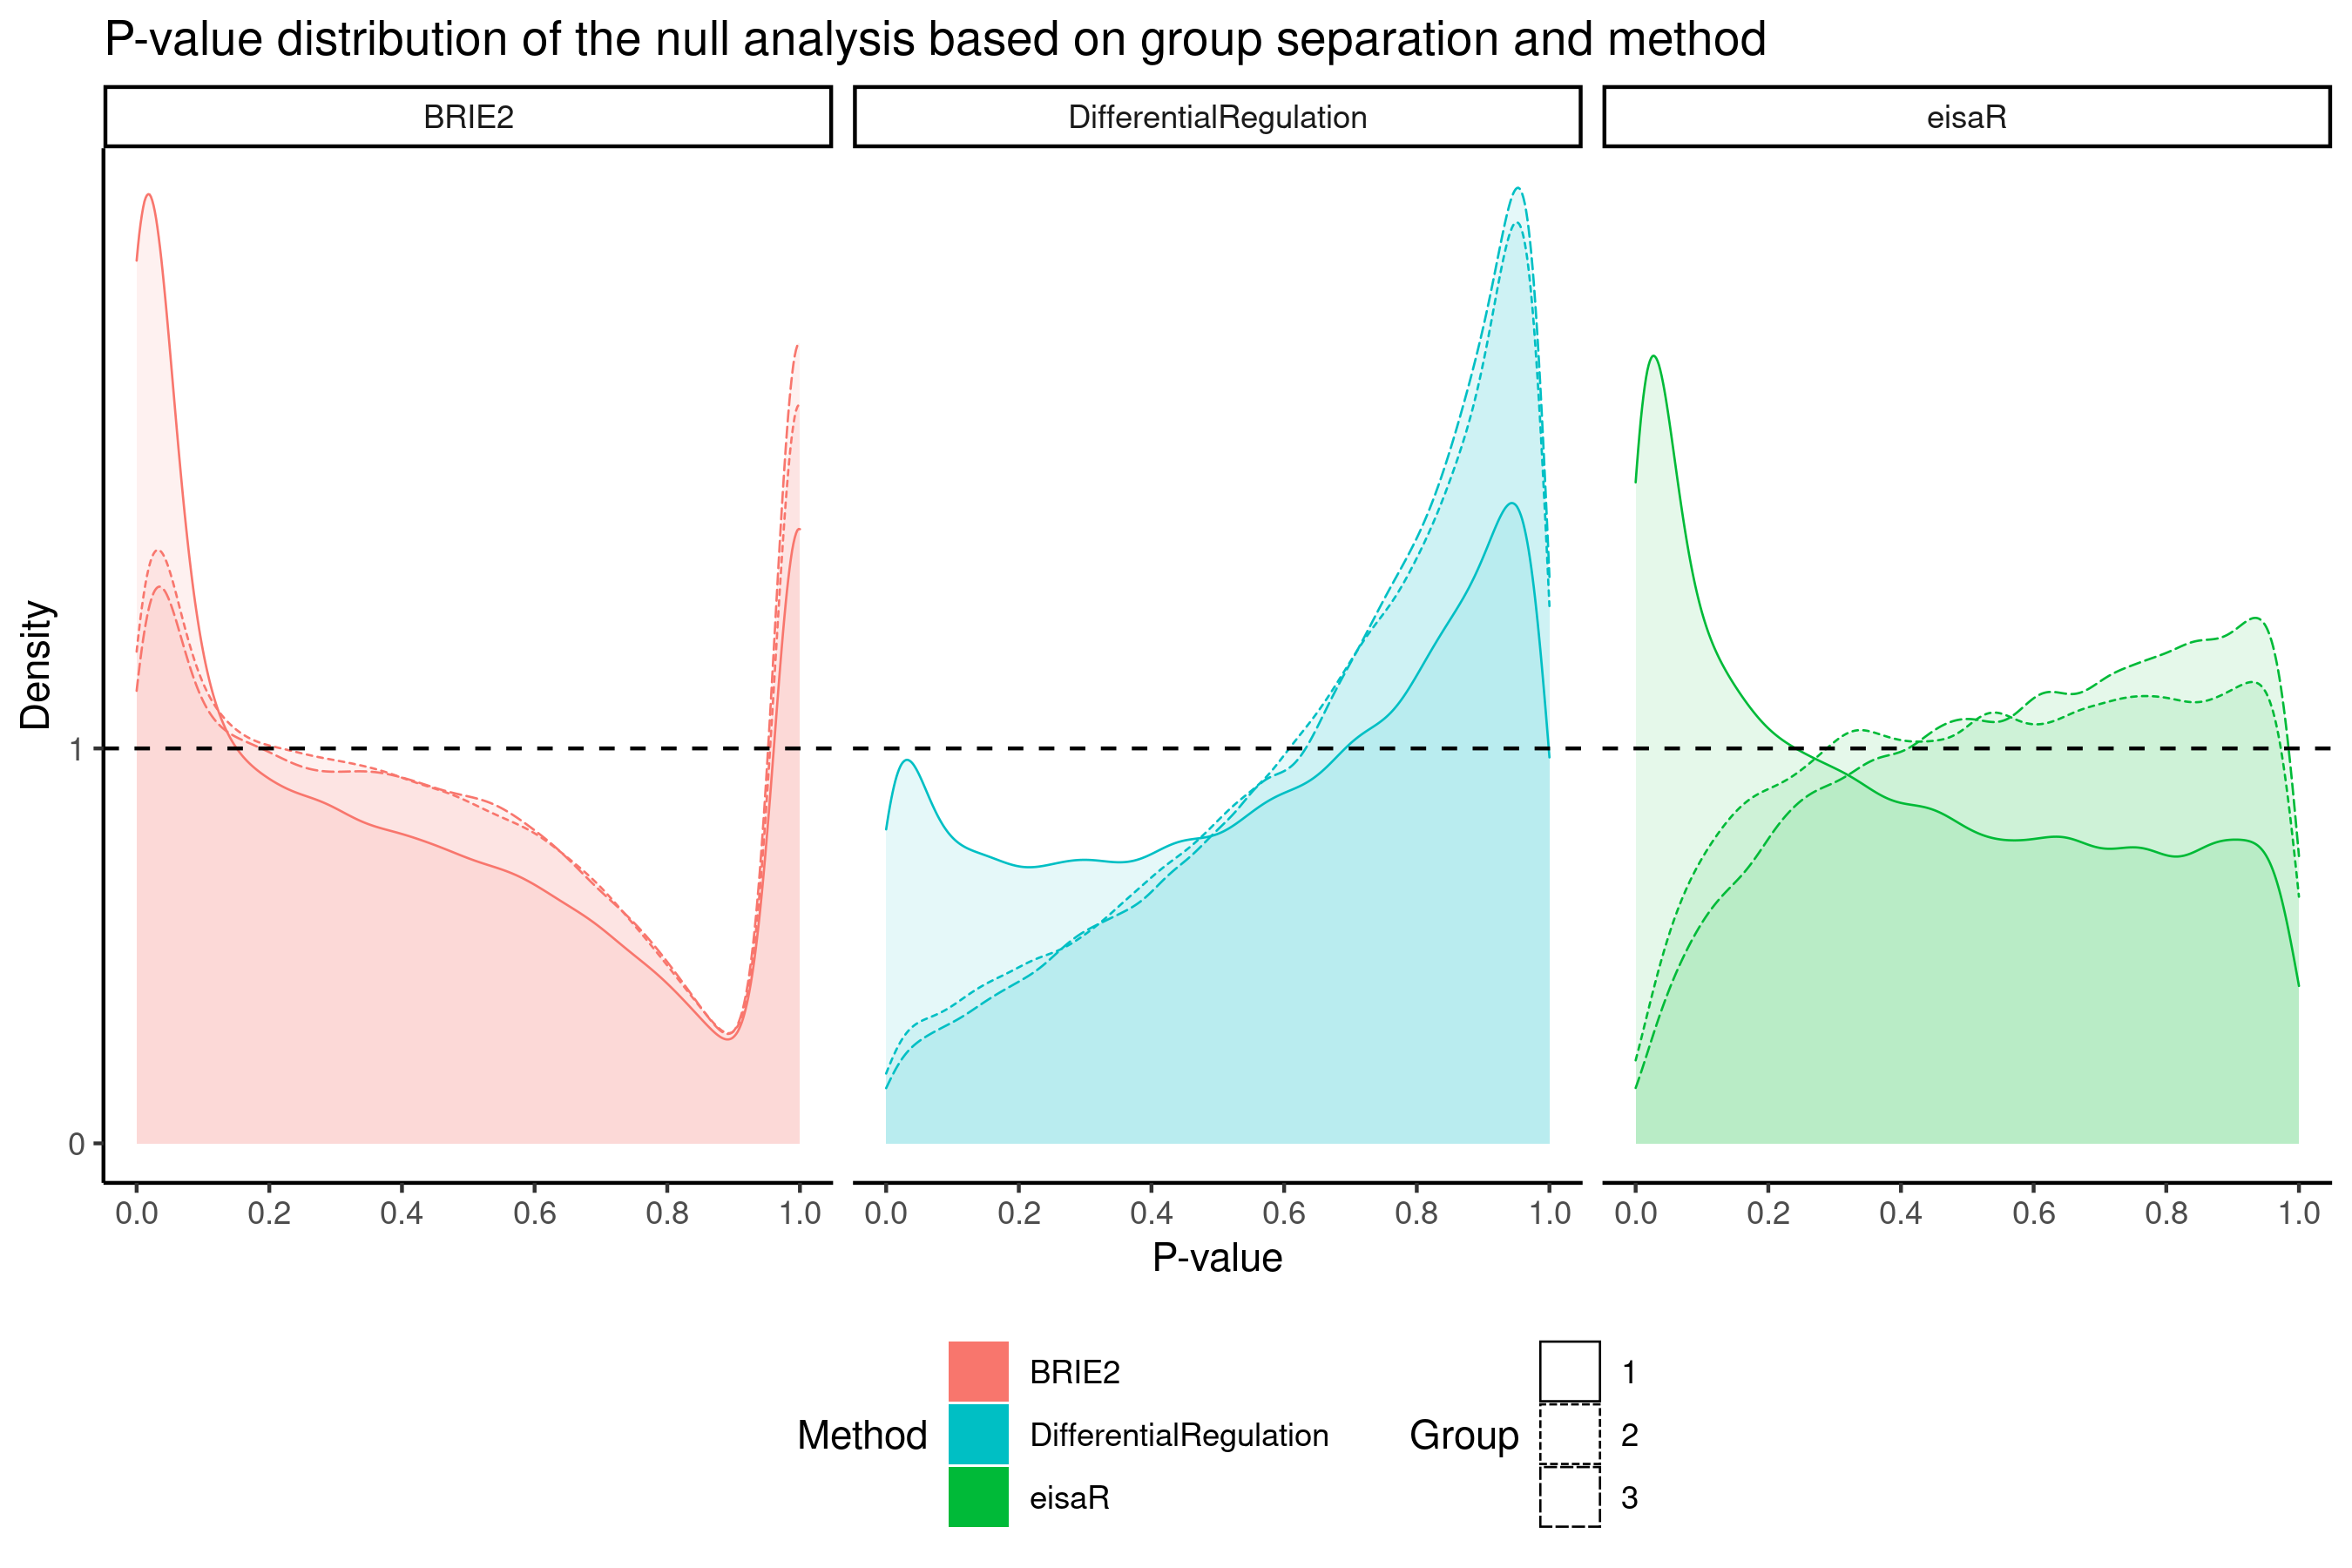
\includegraphics[width=6in,height=3.8in]{../figures/null_analysis/p_value_distribution.png}
\end{center}
\caption{P-value distribution of the methods based on the three possible group separations}
\label{fig:null_p_values}
\end{figure}

Further, we looked into the performance of the models based on the proportion of p-values and FDR values smaller or equal than the conventional significance levels of 10\%, 5\% and 1\%. From Table \ref{tab:p_val} it is shown that \emph{BRIE2} does not control the p-values particularly well as the values are inflated for all three levels. On the other hand, both \emph{DifferentialRegulation} and \emph{eisaR} do not have inflated p-values, whereas \emph{DifferentialRegulation} is a bit more conservative than \emph{eisaR}. Table \ref{tab:fdr} paints a similar picture as \emph{BRIE2} produces by far larger values than the other methods including \emph{DEXSeq}. With FDR values one would usually want the values to be as small as possible. From that convention one can observe that \emph{DifferentialRegulation} controls the FDR better than both \emph{DEXSeq} and \emph{eisaR}, whereas the latter two methods perform approximately equally as good.

\begin{table}[!htb]
\centering
\caption{Proportion of p-values smaller than the proposed significance levels 10\%, 5\% and 1\%}
\begin{tabular}{rrrr}
  \hline
	& 10\% & 5\% & 1\% \\ 
  \hline
	BRIE2 & 0.215 & 0.155 & 0.083 \\ 
  DifferentialRegulation & 0.059 & 0.035 & 0.014 \\ 
  eisaR & 0.108 & 0.065 & 0.026 \\ 
   \hline
\end{tabular}
\label{tab:p_val}
\end{table}

\begin{table}[!htb]
\centering
\caption{Proportion of FDR values smaller than the proposed significance levels 10\%, 5\% and 1\%}
\begin{tabular}{rrrr}
  \hline
	& 10\% & 5\% & 1\% \\
  \hline
	BRIE2 & 0.080 & 0.061 & 0.038 \\ 
  DEXSeq & 0.016 & 0.012 & 0.006 \\ 
  DifferentialRegulation & 0.006 & 0.005 & 0.003 \\ 
  eisaR & 0.017 & 0.010 & 0.004 \\ 
   \hline
\end{tabular}
\label{tab:fdr}
\end{table}
\FloatBarrier

\section{Computational benchmark}
Ultimately, we compared the computational burden of the differential methods excluding alignment and quantification. Alignment and quantification were excluded from the benchmark as all methods use the same input generated from \emph{alevin-fry}, therefore including it would be redundant. The computational benchmark was run on the Null data and averaged across all three possible group separations. All methods were provided three cores on the same machine (internal server) to run the benchmark. However, \emph{BRIE2} uses all cores available on a machine and \emph{eisaR} only runs on one core. Figure \ref{fig:bench_mark} illustrates the average runtime of each differential method in minutes on a square root scaled axis, as there is a large difference in absolute runtime between the methods. From the Figure it is shown that \emph{BRIE2} ran the longest - roughly 2000 minutes. However, we did not run \emph{BRIE2} on a GPU, which is its intended use. The other three methods finished within an hour with \emph{DifferentialRegulation} taking the longest and \emph{eisaR} taking the shortest.

\begin{figure}[!htb]
\begin{center}
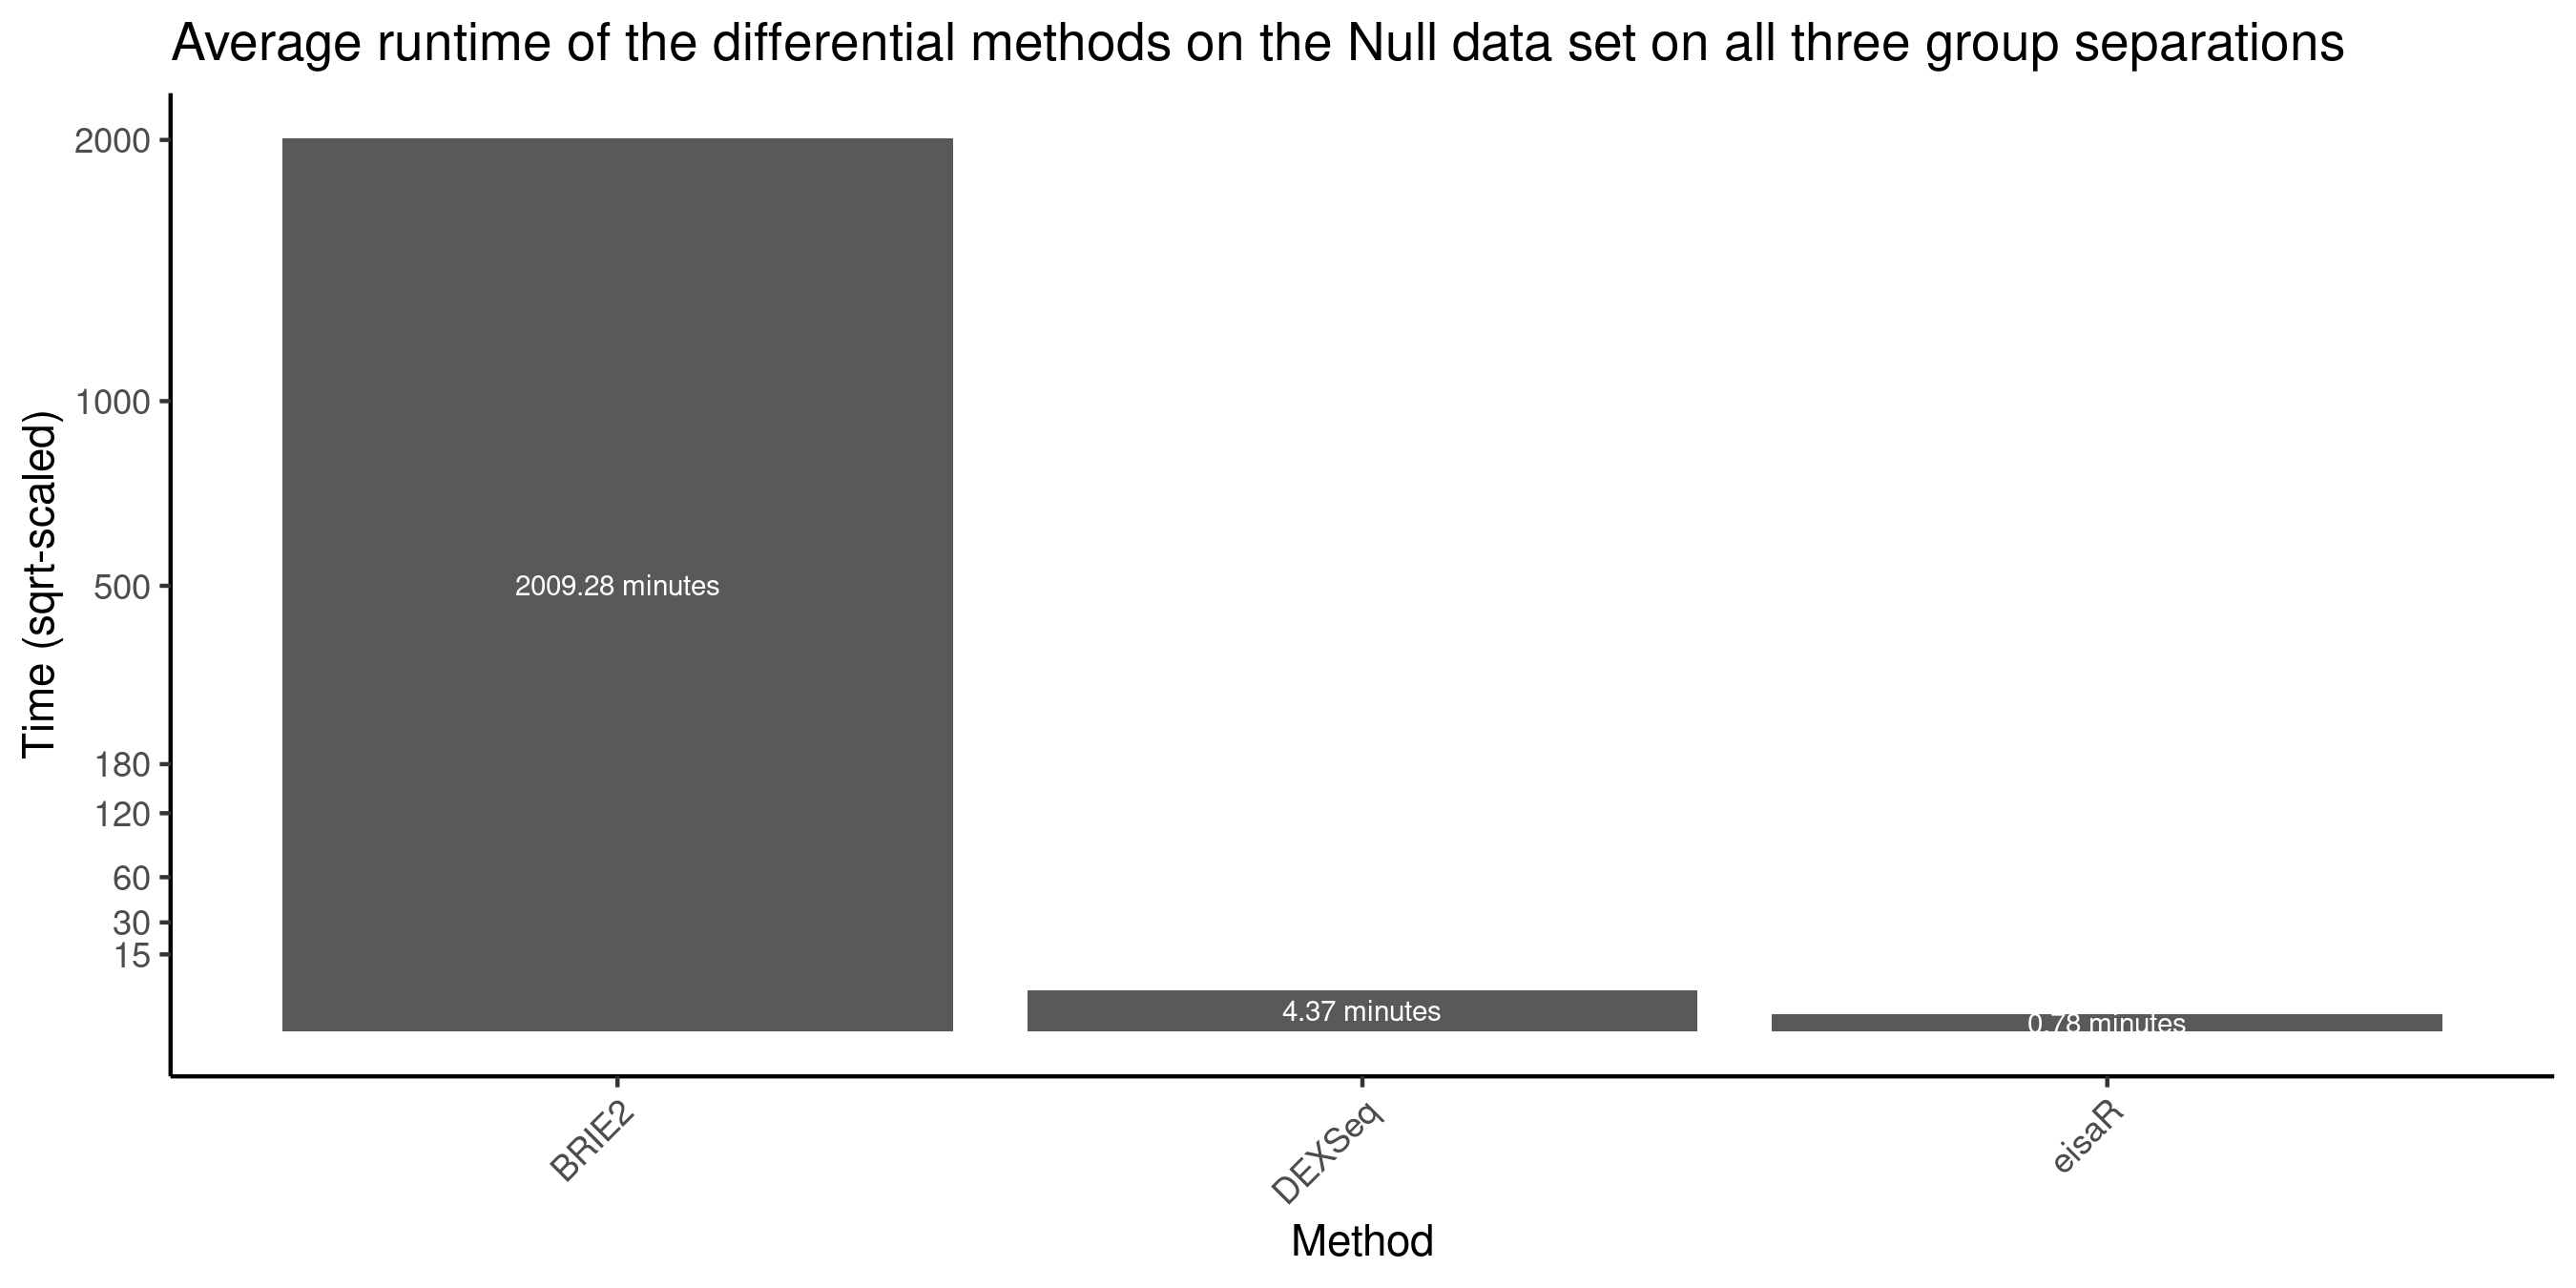
\includegraphics[width=6in,height=3in]{../figures/null_analysis/bench_mark.png}
\end{center}
\caption{Runtime of the differential methods on the Null data averaged across all three possible group separations}
\label{fig:bench_mark}
\end{figure}
\FloatBarrier

\section{Data availability}

\noindent\textbf{Kidney mouse cells} \\
The raw data can be downloaded from NCBI GEO (accession number GSE107585). \\ 
\url{https://www.ncbi.nlm.nih.gov/geo/query/acc.cgi?acc=GSE107585} \\

\section{Code availability}
All code for data preprocessing and analysis associated with the thesis is available at \url{https://github.com/joelmeili/DifferentialRegulation}.
